\documentclass{article}

\usepackage{natbib}
\usepackage{authblk}
\usepackage[utf8]{inputenc}
\usepackage{hyperref}
\usepackage{graphicx}
\usepackage{multirow}
\usepackage{tabularx}
\usepackage{booktabs}
\usepackage{longtable}
\usepackage{appendix}
\usepackage{xcolor}
\usepackage{booktabs} 

\usepackage{times}
\usepackage{latexsym}
\usepackage{floatpag}

\usepackage[parfill]{parskip}
\usepackage[utf8]{inputenc} % allow utf-8 input
\usepackage[T1]{fontenc}    % use 8-bit T1 fonts
\usepackage{hyperref}       % hyperlinks
\usepackage{url}            % simple URL typesetting
\usepackage{booktabs}       % professional-quality tables
\usepackage{amsfonts}       % blackboard math symbols
\usepackage{nicefrac}       % compact symbols for 1/2, etc.
\usepackage{microtype}      % microtypography
\usepackage{graphicx}
\usepackage{natbib}
\usepackage{tabularx}
\usepackage{xtab}

\usepackage{float}   % For the [H] specifier to force placement


\usepackage{geometry}  %this makes the columns wider 
\usepackage{siunitx}
\usepackage{booktabs, makecell}
\usepackage[referable]{threeparttablex}

\title{%The KL3M Dataset:  A Copyright Clean 80TB+ Dataset for Pretraining and Supervised Fine Tuning of Language Models

The KL3M Dataset:  A Copyright Clean 80TB+ Dataset for Pretraining and Supervised Fine Tuning of Large Language Models


}
\author{\normalsize{Michael J Bommarito II,\textsuperscript{1,2} Jillian Bommarito}\textsuperscript{1} \& Daniel Martin Katz\textsuperscript{1,2,3,4}\\
  \textit{\small \textsuperscript{1} Institute for the Advancement of Legal and Ethical AI (ALEA Institute)\\
  \textit{\small \textsuperscript{2} CodeX -- The Stanford Center for Legal Informatics}\\
  \textit{\small \textsuperscript{3} The Law Lab, Illinois Tech - Chicago Kent College of Law}\\          
    \textit{\small \textsuperscript{4} Center for Legal Technology \& Data Science, Bucerius Law School}\\  
  }
}
  
\date{\normalsize{March 13, 2025}}

\begin{document}

\maketitle

\begin{abstract}
{Practically all large language models have been pre-trained on data that is subject to global uncertainty related to copyright infringement, breach of contract, and privacy. In light of this reality, we present the 80TB+ sized Kelvin Legal Large Language Model (KL3M) dataset, the largest collections of pretraining and supervised fine-tuning data which is unencumbered by copyright risk.  In total, KL3M contains over 125 million documents and more than 1.7 trillion tokens.  This paper outlines our approach to creating a dataset free from copyright uncertainty including details on our data sources, and collection and preprocessing methods.  While our data sources are limited to US and certain EU source materials, we open source not only the dataset itself but also the tokenizer, API's and other associated software in order to support further allied development in other jurisdictions.  We believe that this represents a significant step towards developing A.I. systems that are legally and ethically sound, both now and in the face of future regulatory changes.}
\end{abstract}
\section{Introduction}
Over the past decade, there has been significant progress on general-purpose language modeling driven by the application of neural based methods \cite{rumelhart1986learning}\cite{hopfield1982neural} to corpora of increasing larger scales.\cite{brown2020language}\cite{dubey2024llama}\cite{guo2025deepseek}  Leading large language models (LLMs) have displayed significant progress on a range of challenging real-world tasks.\cite{goh2025gpt}\cite{dell2023navigating}\cite{katz2024gpt}\cite{brin2023comparing}

While fewer and fewer question the technical progress of these models' capabilities, the training and use of large language models, however, is not without controversy.   Indeed, there are an emerging range of questions associated with the development of generative A.I. technology.  These objections vary and cover a range of topics including the `openness' of the model creation process and the `toxicity' of the subsequent outputs.\cite{liesenfeld2024rethinking}\cite{longpre2024pretrainer}\cite{bommasani2024foundation}  While these are certainly important issues, far less attention, by contrast, has been paid to use training data collected at scale without respect to the moral and legal rights of its creators.  

Virtually all existing LLMs rely upon the large-scale collection and use of materials that are subject to copyright. Despite various clever efforts to ameliorate such issues at both training \cite{minsilo2024} and inference time \cite{golatkar2024cpr}\cite{ippolito2023preventing}\cite{flemings2024differentially} many leading models can still engage in relatively high levels of potentially infringing behavior.\cite{chen2024copybench}     

There is still the open question of whether notions ``fair use" or ``fair dealing" might serve as a legal defense to this otherwise problematic behavior.\cite{henderson2023foundation}\cite{sag2024fairness}  However, it is worth noting that while ``[M]ore than forty countries with over one-third of the world’s population have fair use or fair dealing provisions in their copyright laws,"\cite{band2013fair} the interpretation of such principles can vary significantly across jurisdictions.\footnote{It is worth noting that although some model providers are offering ``fair use'' as a defense to their data collection practices, many such organizations are also inherently acknowledging the property rights of creators by entering into licensing deals.} 

In light of this reality, we set out on an alternative path - one that is rooted in a rigorous data collection and curation processes designed to respect traditional legal and ethical frameworks.  In this paper, we present the Kelvin Legal Large Language Model (KL3M) dataset, tokenizer, software, and APIs. These assets, open-sourced and maintained by the ALEA Institute,\footnote{\textit{See} Institute for the Advancement of Legal and Ethical AI (ALEA Institute) \url{https://aleainstitute.ai/} } represent one of the largest collections of pretraining and supervised fine-tuning data unencumbered by copyright risk.  We outline a framework for determining permissibility of content usage that can be employed by anyone who wants to gather or audit training data for model training or fine-tuning. In addition, we enhance the data provenance visibility of the KL3M dataset by providing Dublin Core metadata for all data in the dataset.\cite{park2009dublin}

%Thus, in the following sections, we will detail our data sources, collection process, preprocessing methods, and the characteristics of the resulting dataset. We will also discuss the implications of our work for future A.I. development in the context of the broader legal and ethical landscape.



%Our approach aims to circumvent the need for reliance on fair use arguments by ensuring all data in the KL3M dataset is either in the public domain or explicitly licensed for unrestricted use.

%In light of this reality, we set out on an alternative research agenda - one that is rooted in legal and ethical practices that are free of doubt. Our primary contribution to a space already saturated with datasets is the research into and development of a path that is free of reliance on the "fair use" argument that is often relied upon for model training.


%With over 30 copyright lawsuits against AI companies currently in progress in the US alone, the need for legal precedent on the matter of copyright infringement and model training is clear. The outcome of these cases will likely establish whether the argument for "fair use" in model training is a viable one. 

%However, regardless of what one believes about the legal and ethical questions underlying this uncertainty, there is no denying the existence of the many lawsuits and investigations ongoing in major jurisdictions.

\section{Copyright and Generative A.I.}
\subsection{Brief Overview of Copyright}
Copyright is sometimes described as a `bargain’ where creators receive, exclusive rights to their works for a specific period of time, in exchange for the public eventually gaining free access to those works after the copyright term expires.\cite{patterson1991nature} Although all materials will eventually reach the public domain, creators may, during their period of exclusive ownership, choose to make their works available to others via licensing at a scope of their choosing.  There is a wide continuum of popular copyright licenses including MIT, Apache, GNU GPL, AGPL as well as various flavors of Creative Commons licenses.\cite{metzger2015free}  Such licenses provide a wide degree of latitude for creators to control the scope of how their respective works are used.  

In the internet era, many individuals and organizations have chosen to make their otherwise copyrighted works available online for the scope delimited use of others. Through various platforms such as \textit{Github} (computer code), \textit{Getty Images} (image licensing), \textit{YouTube} (video repositories) or directly through personal websites, the internet has arguably facilitate the most extensive period of information sharing in all of human history.  At the same time, there have also been disputes surrounding the extent to which digitized information could be made available to users. Indeed, controversy has been `part and parcel' of the internet era including major clashes over projects such as \textit{Google Books}\cite{samuelson2009google} and file sharing sites such as \textit{Napster}.\cite{rayburn2001after}  

\subsection{Copyright and A.I. Data Collection}
Although disagreement over proper the scope of copyright is not new, the advent of LLMs has brought with it heightened concerns about the acquisition and use of otherwise copyrighted source materials.\cite{samuelson2023generative}  Virtually all model providers and large scale datasets collected in furtherance of building LLMs have ignored both the website terms of service in the scraping of websites as well as licensing restrictions attached to the respective content collected.\cite{longpre2024large}  As a result, the internet has seen a rise in restrictions upon sharing including a range of efforts to prevent data from being used in the training of A.I. systems.\cite{longpre2024consent}  
Individual creators and content based organizations threatened by A.I. systems that arguably undermine creators future economic prospects have begun to place additional restrictions on their works in an effort to limit reuse, redistribution, and commercial use of their copyrighted materials in the building of A.I systems.\cite{longpre2024consent}

Since the advent of the large-scale public internet, there have been a variety of public and commercial efforts to track its development and growth.\cite{mcmurdo1995internet}\cite{alnoamany2014and}  Much of those efforts centered around ``search'' and helping route individuals to relevant webpages. However, indexing the internet is not the precisely akin to full collection of content.  For example, in the early years of the current millennia, linguists were slow to include large-scale web content given anxiety over copyright in the underlying source materials.\cite{ide2002american}  While some of such materials did eventually make their way into important corpora,\cite{ide2008american} the specter of legal restrictions caused some to limit their use of materials obtained from the internet. 

Other groups, however, were far less motivated by such concerns and began to look at the internet as a premier source of data.  Beyond mere tracking and indexing, internet data has been subjected to various large scale collection efforts including graph data, images, metadata and the underlying text.\cite{buck2014n}\cite{leskovec2016snap}\cite{deng2009imagenet}  \textit{Common Crawl}\cite{smith2013dirt} one of longest standing efforts to collect web-scale data has served as a foundational dataset in many early LLMs. \textit{Common Crawl} and subsequent efforts to build large-scale A.I. training datasets such as the \textit{Colossal Cleaned Common Crawl} (C4)\cite{raffel2020exploring}, \textit{The Pile}\cite{gao2020pile} and \textit{Dolma}\cite{soldaini-etal-2024-dolma} are replete with copyrighted data. 

%Common Crawlhas been cited in thousands of academic articles \footnote{https://github.com/commoncrawl/cc-citations/} 

As noted earlier, the collection and distribution of such materials relies upon ``fair use'' as a justification. ``Fair use'' is fact-specific inquiry meaning that whether a particular use of copyrighted material is considered ``fair use'' depends upon specific details that must be evaluated on a case-by-case basis.  For example, when an academic institution or other non-profit type research organization collects data for research purposes that activity would likely be ``fair use.''  Yet, if that same dataset were deployed for subsequent commercial use by an entity whose direct or indirect aim is to undercut the commercial viability of the original creator (\textit{e.g.} coder, artist, author or musician) that activity might not be characterized as ``fair use.''  Even if ``fair use'' were not deemed to cover a particular usage, it is possible that royalty system including perhaps compulsory licensing might be a vehicle for rewarding creators\footnote{A market based licensing and royalty system including perhaps a compulsory licensing would be more ethical than allowing individuals and organizations to seize the creative works of others without \textit{any} compensation. Such ideas are explored in a recent report released by the U.S. Copyright Office.\cite{Jaffe2025}} while still allowing for innovation in A.I. model building to continue.\footnote{In a letter sent to the White House Office of Science and Technology (OSTP), OpenAI argued that ``[A]pplying the fair use doctrine to AI is not only a matter of American competitiveness — it’s a matter of national security ... If the PRC’s developers have unfettered access to data and American companies are left without fair use access, the race for AI is effectively over.''\cite{OpenAI}  While clarity regarding the legal treatment of this question would be helpful, it is far from clear that the requirement of royalty payments to creators would materially impair the rate of innovation.}

Certain scholars working with datasets such as \textit{Common Crawl}, \textit{C4} and \textit{The Pile} have recognized the looming copyright questions surrounding these efforts.\cite{schafer2016commoncow}\cite{habernal2016c4corpus}  For example, authors of the recently released  \textit{Dolma} dataset stated ``that the legal landscape of A.I. is changing rapidly, especially as it pertains to use of copyrighted materials for training models.''\cite{soldaini-etal-2024-dolma}  However, they still chose to distribute their dataset because the ``sources were publicly available and already being usedin large-scale language model pretraining (both open and closed).'' 

This perspective is emblematic of much of the broader literature on ethics in A.I. where there has been much greater focus on questions of model ‘openness’ and `A.I. alignment' than respect for the scope of the moral and legal rights of creators.  Although issues of transparency and model toxicity are important, they are far from the only consideration worthy of attention.  

Most recently, the \textit{Common Corpus} dataset\cite{arnett2024toxicity}  was released on the \textit{Hugging Face} platform.  The dataset was promising as the authors claimed that the compilation ``contains only data that either is uncopyrighted or permissively licensed.''  Unfortunately, the rhetoric surrounding the dataset does not match its reality.  Although the authors recognize the ethical and potential legal issues associated with scraping data without the consent of the data creator, the authors provide very little description of their copyright audit process.  It turns out that even a cursory inspection of the dataset reveals a significant volume of copyright materials contained therein. 


%As noted earlier, the extant literature has in part begun to acknowledge and confront some of the potential ethical and legal challenges associated with the construction of modern LLMs. Much of the focus, however, has been directed at questions of model ‘openness.’   While ‘openness’ is certainly an attractive property of a development pipeline, it is insufficient without a clear analysis of the ethical and legal requirements.  

%by contrast, does not even pretend to care about the rights of content creators.  Instead, it is includes components such as Books3, Pile-CC, Github and Wikipedia.   FOOTNOTE  [[ The use of Wikipedia (whose pages feature a wide range of licenses selected at the behest of users) is almost certainly problematic at scale.  The Wikimedia foundation lacks the legal authority to change the license terms for  ]]


%As noted earlier, the extant literature has in part begun to acknowledge and confront some of the potential ethical and legal challenges associated with the construction of modern LLMs. Much of the focus, however, has been directed at questions of model ‘openness.’   While ‘openness’ is certainly an attractive property of a development pipeline, it is insufficient without a clear analysis of the ethical and legal requirements.  

%The authors of Common Corpus dataset recognize that it is unethical (and arguably illegal) to scrape (data) without the consent of the data creator.   While the authors claim that the dataset ‘contains only data that is uncopyrighted or permissively licensed,’ the authors provide no description of the process by which such copyright analysis was conducted.  And in fact, even a minimum inspection reveals a significant amount of copyright materials contained with the dataset.   

%The Pile, by contrast, does not even pretend to care about the rights of content creators.  Instead, it is includes components such as Books3, Pile-CC, Github and Wikipedia.   FOOTNOTE  [[ The use of Wikipedia (whose pages feature a wide range of licenses selected at the behest of users) is almost certainly problematic at scale.  The Wikimedia foundation lacks the legal authority to change the license terms for  ]]

   





\section{Copyright Clean Collection Process}
We believe that the continued development and use of AI systems should be predicated on such systems being both legally and ethically compliant, both in the current environment and in the wake of future regulatory and legislative changes.  In this section, we introduce the Kelvin Legal Large Language Model (KL3M) dataset, the largest dataset developed to date that respects the moral and legal rights of copyright holders. Our approach aims to circumvent the need for reliance on ``fair use" arguments by ensuring all data in the KL3M dataset is either in the public domain or explicitly licensed for unrestricted use.


\subsection{Copyright Filtration Process}
To build KL3M, we developed a multi-part filtration process designed to determine whether a given data source may be used without significant restriction. The test is based on a series of conditional assessments: if the data passes a test, we include it in the KL3M dataset; if the data does not pass the test, we move on to the next test. Data that does not pass any of our tests is not included in the KL3M dataset.  We describe the process below but also highlight the steps in Figure \ref{fig:CopyrightFlowchart} below.

\begin{figure}[ht!]
\centering
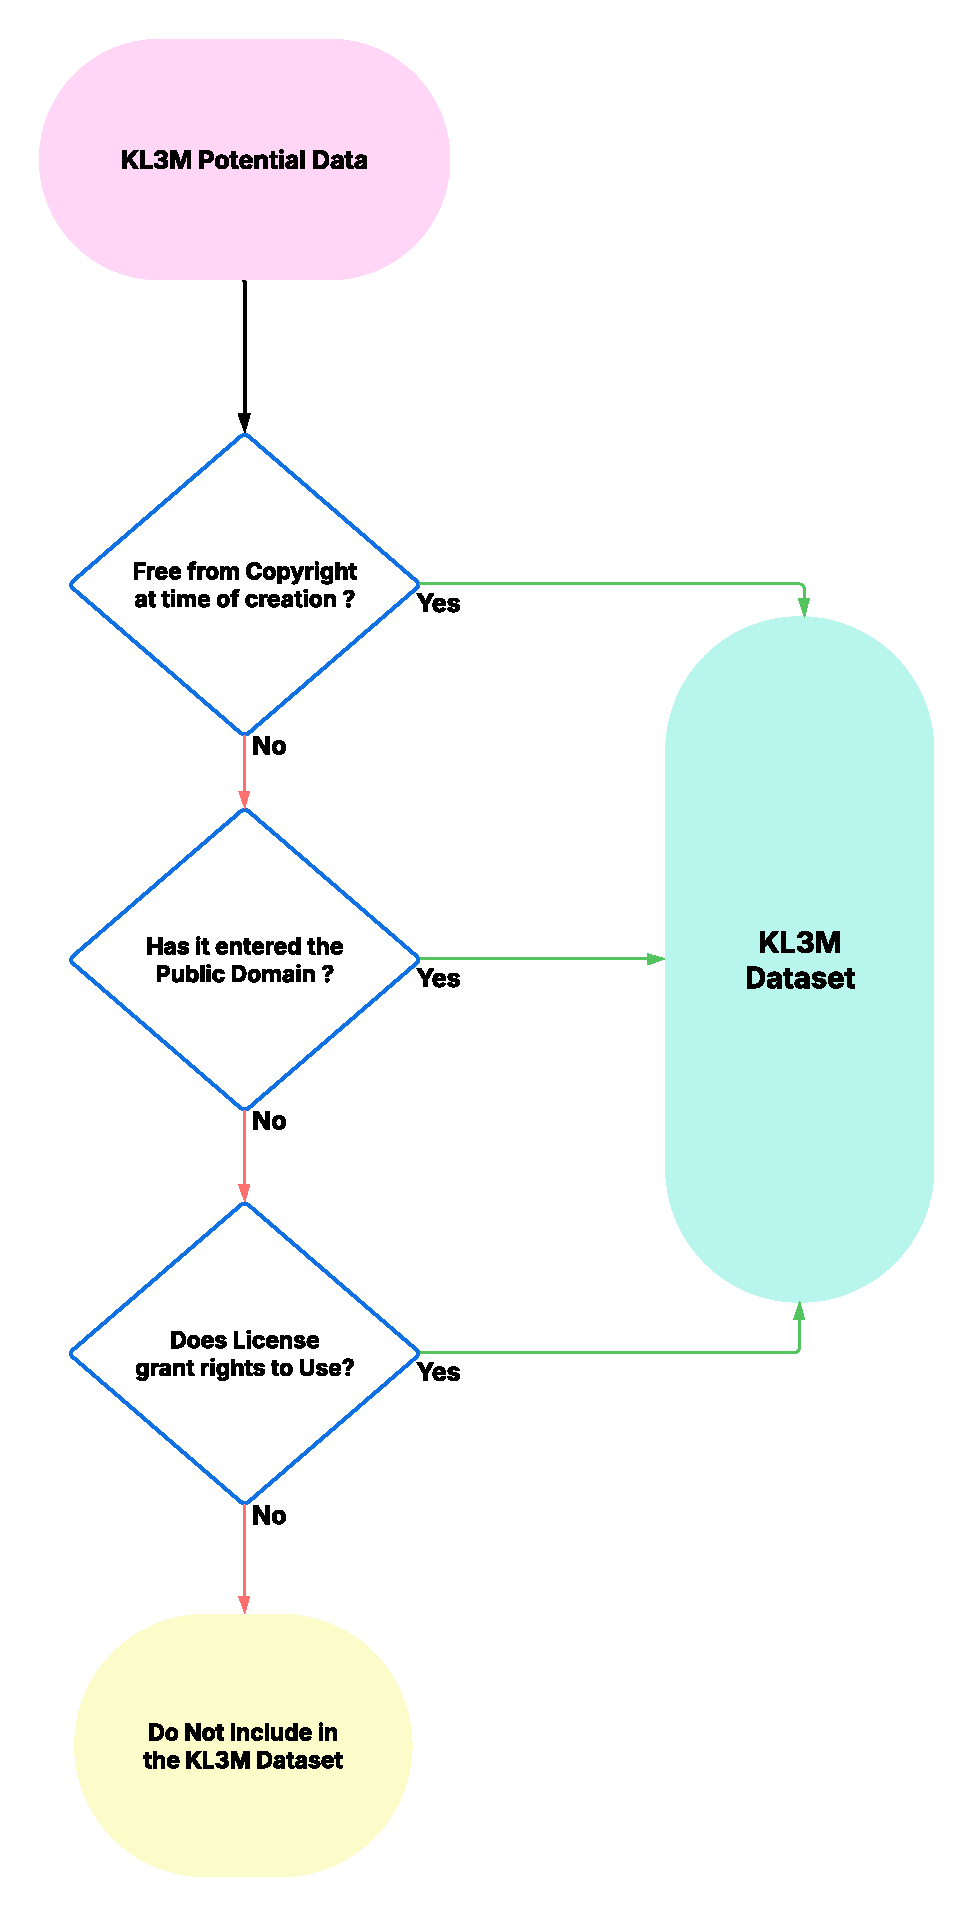
\includegraphics[width=70mm]{CopyrightFlowchart.pdf}
\caption{Overview of the Copyright Filtration Process}
\label{fig:CopyrightFlowchart}
\end{figure}

\subsubsection{Test 1 - Free from Copyright Protection}
Our first test is to determine whether the content is free from copyright \textbf{at the time of its creation}. A substantial percentage of content contained within the KL3M dataset meets this test and was thus eligible for inclusion.

Works of the United States government, for example, are not eligible for copyright protection under 17 U.S.C. § 105 (``Copyright protection under this title is not available for any work of the United States Government").  Specifically, work created by a federal government employee or officer is in the public domain, provided that the work was created in that person’s official capacity. 

A separate but related concept is the ``government edict doctrine."  This doctrine, developed through the common law, denies copyright protection to official ``government edicts."\footnote{The doctrine is long standing and dates back to \textit{Wheaton v. Peters}, 33 U.S. (Pet. 8) 591 (1834) and has most recently been addressed in \textit{Georgia v. Public.Resource.Org, Inc.}, 590 U.S. 255 (2020).}  The doctrine exists to effectuate the principle that citizens must have unrestrained access to the laws that govern them.  The ``government edict doctrine" allows for the publication of various legislative and judicial pronouncements including judicial opinions.  As noted by the U.S. Copyright Office, the doctrine extends to ``all legislative enactments, judicial decisions, administrative rulings, public ordinances, or similar types of official legal materials.''\footnote{U.S. Copyright Office, Compendium of U.S. Copyright Office Practices, §313.6(C)(2) (3d ed. 2017)}

Most but not all countries follow this doctrine. For example, we had hoped to include certain UK legal sources within the KL3M dataset but limitations embedded in the Open Justice License (OJL)  surrounding the ``computational analysis of the information'' prevented us from including such UK data at this time.\footnote{\textit{See} Open Justice License (OJL) \url{https://caselaw.nationalarchives.gov.uk/open-justice-licence}} 

\subsubsection{Test 2 - Public Domain Materials}
In our second test, we determine whether content has \textbf{entered into the public domain} or its equivalent, such as a Creative Commons - No Rights Reserved (CC0) license where no rights are reserved. There are several ways that content, once subject to copyright, could thereafter enter the public domain.  Most notably, although the amount of time has changed over the years, copyright is always a temporary grant of exclusive rights for a defined period of time.  Therefore, once that designed time has lapsed, the work automatically enters the public domain.  For example, while we would prefer to include the most recent Twelfth Edition\cite{black2024} published in 2024, we instead include in the KL3M data the Second Edition of Black's Law Dictionary originally published in 1910.\footnote{Black's Law Dictionary contains definitions of specialized legal terms. The substantive meaning of many such terms has not changed for many years.} 

Other information can enter the public domain as part of a particular legal process.  For example, we include granted patents in KL3M as patents are typically not subject to copyright restrictions.  As noted by the USPTO, ``[P]atents are published as part of the terms of granting the patent to the inventor.''  Absent a limited set of circumstances, ``the text and drawings of a patent are typically not subject to copyright restrictions.''\footnote{\textit{See} USPTO Terms of Service \url{https://www.uspto.gov/terms-use-uspto-websites}}  
%Following the terms We include also include public comments on regulatory submissions as part of notice and comment rule making within the KL3M dataset. 

One additionally important vehicle for adding information to the public domain is the US Federal Depository Library Program (FDLP). The Federal Depository Library Program (44 U.S.C. § 19), administered by the U.S. Government Publishing Office, was established to ensure that the American public has access to Government information. 44 U.S.C. § 1911 states that ``[D]epository libraries shall make Government publications available for the free use of the general public.''  Although many of the documents required extensive pre-processing in order to be usable, the FDLP is a very large source of useful information for KL3M.  

\subsubsection{Test 3 - Minimally Encumbered Content with Clear Rights to Copy, Modify, and Redistribute}
If the use of content is not otherwise permissible following the two prior tests, the final test is to determine whether the \textbf{license attached to the content grants a user the right to copy, modify, and redistribute the content without significant restriction}.  As highlighted in Figure \ref{fig:CopyrightFlowchart}, if content fails this final test, we did not include it in the KL3M dataset.

While CC0 or No Rights Reserved is, of course, the most unencumbered form of license, there are a range of other content licenses that might theoretically be considered for inclusion.   Overall, we evaluated content with the following license types using the reasoning below:

\begin{itemize}
\item CC0: included given content is shared with No Rights Reserved 
\item CC BY: included as the attribution is not overly burdensome (particularly in the case of an institution as author)
\item CC BY-SA: excluded due to the uncertainty around meeting share-alike obligations in the context of a Large Language Model\footnote{While we plan to meet the Share-alike requirements in the full Open Source release of KL3M, we recognize that others might consider this to be major encumbrance upon utilization.}
\item CC BY-NC: excluded due to non-commercial limitation
\item CC BY-NC-SA: excluded due to non-commercial limitation and uncertainty around meeting share-alike obligations
\item CC BY-ND: excluded due to limitation on derivative work
\item CC BY-NC-ND: excluded due to non-commercial and derivative work limitations
\end{itemize}

In general, in the context of content created by an institution, we believe an attribution requirement is only a very modest restriction upon downstream use.  For example, content released by the European Commission under 2011/833/EU is only minimally encumbered as it merely imposes an ``obligation for the reuser to acknowledge the source of the [Commission's] documents.''\footnote{\textit{See} On the reuse of Commission documents \url{https://eur-lex.europa.eu/eli/dec/2011/833/oj/eng}}  Similarly, in most cases, compliance with the attribution requirement set forth in the Creative Commons License (CC BY) is similarly straightforward.  

However, there are arguably some nuances and complexity in the context of non-institutional authors. Indeed, some of the most fruitful data that we might consider for inclusion could not meet our goal of building a dataset that was relatively unencumbered.  For example, despite its inclusion in other training datasets such as \textit{Colossal Cleaned Common Crawl} (C4) \cite{raffel2020exploring}, \textit{The Pile} \cite{gao2020pile}, \textit{Dolma} \cite{soldaini-etal-2024-dolma} and \textit{Common Corpus} \cite{arnett2024toxicity}, \textit{Wikipedia} and many other knowledge commons are arguably encumbered by the ``copyleft'' licenses that the community has chosen. 

From a historical perspective, \textit{Wikipedia} content was originally licensed under the GNU Free Documentation License  (GFDL).\cite{roessing2010authorship}  Today, it is arguably licensed under CC BY SA which carries with it not only a share alike (SA) requirement but also an attribution requirement (BY).  We contacted the \textit{Wikimedia Foundation} to ascertain their perspective regarding the scope of attribution that they believe would be required to use the content on \textit{Wikipedia}.  Specifically, given the millions of total contributors who at some point have authored content on \textit{Wikipedia}, we wanted to determine whether they believe that a general attribution statement or a specific attribution statement was required.   

In the context of building or fine-tuning large language models, a general attribution statement highlighting the respective input sources to a given dataset or model is relatively easy to provide.  However, specific attribution to the specific work or works that gave rise to a \textit{specific model output} is a difficult if not impossible technical challenge. It was the Wikimedia Foundation's position that ``providing a general notice to customers would not be an adequate solution to compliance.''  While Wikimedia's interpretation of the CC BY SA requirement is not the final word on this important legal question, we did feel comfortable including this content given it would significantly encumber downstream usage.\footnote{It is not clear how \textit{any} model creator could comply with a \textit{specific attribution} requirement given current technical limitations. At best, one could construct a system to assign \textit{statistical attribution} by assigning attribution through some sort of 
potential \textit{n-gram} based matching or other higher-order statistical style inference.  However, from an attribution perspective, this would undoubtedly produce false positives as well as false negatives.}  

In addition to the Wikimedia Foundation's interpretation of the (BY) requirement, \textit{Wikipedia} has a share alike (SA) requirement which like other ``copyleft'' licenses carries with it the requirement that downstream users make any new works they create with the original content available on the same terms as the original content.\cite{carver2005share}\cite{lessig2004creative} Specifically, the human-readable summary of the \textit{Wikipedia Creative Commons Attribution-ShareAlike 4.0 International License} states ``if you alter, transform, or build upon this work, you may distribute the resulting work only under the same, similar or a compatible license.''\footnote{\textit{See} Wikipedia Creative Commons Attribution-ShareAlike 4.0 International License \url{https://en.wikipedia.org/wiki/Wikipedia:Text_of_the_Creative_Commons_Attribution-ShareAlike_4.0_International_License}} Given these restrictions, it is unclear how \textit{any} model creator could use \textit{Wikipedia} data without making their model fully available under similar CC BY SA / GFDL terms.\footnote{Relying solely on the ``fair use,'' virtually \textit{all} model providers have used \textit{Wikipedia} data in constructing their models. To our knowledge, however, none of them have followed the attribution requirement (BY) as interpreted by the \textit{Wikimedia Foundation} and most do not come close to complying with \textit{Share Alike} (SA) requirement.}  

%\footnote{Similarly, the Wikipedia Creative Commons Attribution-ShareAlike 3.0 International License states ``If you remix, transform, or build upon the material, you must distribute your contributions under the same license as the original.} 

%It should be noted that book platforms such \textit{OpenStax} have similar issues where many individual authors have selected licenses that significantly impair subsequent use.   

%While institutional attribution requirements for content such as EU sources under 2011/833/EU, providing a general notice to customers would not be an adequate solution to compliance. 

%Unlike the institutional attribution requirements for content such as EU sources under 2011/833/EU, copyleft licenses such as GNU FDL and CC BY SA.

%While the United Kingdom's Open Government License (OGL) appears to also have only limited restrictions, access to case law falls under the Open Justice License (OJL).  As noted above the presence of the ``computational analysis'' clause counseled us against including such information.  

%\subsection{Technical Description}
% Add details about the technical process of retrieving the texts here when available

\subsection{Fairly Trained Certification}
In 2024, the KL3M dataset was audited by the independent non-profit \textit{Fairly Trained}.\footnote{\textit{See} Fairly Trained \url{https://www.fairlytrained.org/} }  \textit{Fairly Trained} is a non-profit certification and auditing organization supported by many creators which is devoted to the certification of models that uphold the highest standards of respect for copyright.  

In certifying a model or dataset as \textit{Fairly Trained}, we were required to provide the provenance of each source contained within the dataset including a detailed review of our KL3M Copyright filtration process.  In addition, we needed to demonstrate any models or libraries we leveraged in the data collection, curation, processing steps were also not built upon the unauthorized use of third party content. After an extensive audit process, the KL3M dataset was the first large language model dataset ever to be certified as \textit{Fairly Trained}.   




%\textcolor{red}
%{DISCUSS KL3M vs other datasets on ALEA Site and the idea that the audit caused us to remove things -- podcasts, certain UK Data, etc. }
%\textcolor{black}

\subsection{Personal Information Considerations}
Personal information instances within the KL3M dataset generally arise from their inclusion in documents that are a matter of the public record or that are works of the government. As a result, the personal information that could theoretically be obtained through a review of the KL3M dataset is already publicly available.

We follow the approach of \textit{CourtListener} and the Board of Directors of \textit{The Free Law Project}.\footnote{\textit{See} CourtListener \url{https://www.courtlistener.com/} and the Free Law Project \url{https://free.law/}} in managing the tension between privacy and the public interest. Documents are only removed from the database under explicit court order.

\subsection{Current Jurisdictional Coverage of KL3M}
We chose to focus on content regulated by US and EU law due to our familiarity with these jurisdictions and the legal intricacies of intellectual property rights. We recognize that this limited coverage does not address much of the world's population and languages, but we hope that the process and tests that we have outlined in this paper as well as the associated infrastructure we have open sourced will enable others to create similar datasets for additional jurisdictions.



%\subsection{Regulatory Compliance Considerations}
%Add text about how this dataset will better enable developers to meet regulatory obligations, particularly with respect to transparency
\section{Overview of KL3M Collection Process}
In developing the Kelvin Legal Large Langugage Model (KL3M), we sought to collect and curate a large body of information which was free from the specter of copyright infringement. As opposed to broad data collected from the internet writ large, we sought to identify sources of high quality information, free from copyright concerns that were reasonably available online.  Governmental data, thus currently represents the vast majority of data within the Kelvin Legal Large Language Model (KL3M) dataset. As an output of the growth of the modern regulatory state,\cite{katz2020complex}\cite{coupette2021measuring} various components of government produce very large bodies of relatively high-quality information content.  In addition, various legal and regulatory processes require individuals and organizations to draft and submit various forms of information to government officials, often with guidance and oversight by lawyers, accountants and other professionals.  
%This led us to primarily focus on information produced by or otherwise made available by government(s) as among other things such data is much higher quality than typical internet data.  

While the substantive quality of many forms of governmental data is quite high, the organization and accessibility of such information is not always nearly as strong.  Although governmental and other related data has slowly made it way into the digital world, the mere digitization of governmental information or work product has not always allowed the public to obtain the crucial information they need.  Poorly designed websites, a lack user-friendly navigation and outdated and inconsistent digital platforms are just some of the challenges faced by individuals engaging with public sector information systems.  We faced these very challenges in collecting and curating the KL3M dataset. Although much of this data is theoretically accessible, it is often stored in various inconsistent formats which make cross-functional access very difficult even in discrete amounts (let alone at scale). 

In this section, we begin by discussing trends in modeling building while providing some exemplars of the wide-ranging content contained within the KL3M dataset.  Next, we detail our efforts to collect, pre-process and organize this vast and diverse corpora.  Finally, we provide a high level overview of the distribution of sources contained within the current version of the Kelvin Legal Large Language Model (KL3M) dataset. 
  
\subsection{Breadth and Quality of Tokens Might Be What You Need}
One challenge in building modern language models is to have both scale and a diversity of pre-training information content to cover the broad conceptual space of potential user queries.  Users might want to ask a model to explain a scientific question, determine how best to cook a particular recipe, look to draft some long-form prose or perhaps even ask questions about how to sublease their apartment.  The prevailing approach to cover the broad conceptual space of potential user queries is simply to scale models to increasing large scales.\cite{kaplan2020scaling}  ``Chinchilla'' and other related scaling laws have encouraged model builders to pre-train on the maximal amount of available pretraining data.\cite{hoffmann2022training}\cite{pearce2024reconciling}.  As such, most developments in LLMs have been focused on the use of various collections of internet and so called ``publicly available'' data to build larger and larger language models. 

Undoubtably, the sheer power of scale has delivered some fairly remarkable results. Engineering, however, is not only about performance, it is also about cost.\cite{Krishna2025}  Thus, an alternative strain of work has focused upon how to cost effectively train models using distillation and other related techniques.\cite{guo2025deepseek}\cite{zhang2024tinyllama}\cite{javaheripi2023phi} The scaling laws upon which the field was once fixated have arguably given way to a more nuanced perspective where token diversity, token quality and test time inference scaling are also an important part of the overall calculus.\cite{snell2024scaling}\cite{yu2024makes}  

\subsection{The Incredible Expanse of Government Work Product}
Legal and regulatory processes implicate a wide variety of pursuits and fields of human endeavour.  Thus, taken as a whole, the work product of governments and governmental processes covers a significant amount of intellectual territory.  While certainly not covering every topic that a user might find interesting, information from governments covers a surprising amount of the broader conceptual space.  Laws, regulations, scientific reports, food safety bulletins, environmental impact assessments, public health guidelines, statistical reports, press releases, disaster preparedness plans, government contracts and certain private contracts, judicial opinions, public commentary, military directives, food and drug recalls, transportation safety reports, economic forecasts, patent filings, congressional testimony, securities filings, census data reports are just some examples of the outputs associated with the governmental work product and governmental processes.  

KL3M features a wide variety of question and answer pairs, professional dialogues, formal definitions of key terminology and parallel assessment documents in multiple languages.  It is quite difficult to fully characterize the incredible expanse of topics and materials contained therein.  Appendix I highlights the KL3M Data Gallery, an online exploration tool which allows users to review millions of sample documents drawn from the broader KL3M dataset.  However, consider Figure \ref{fig:KL3MImages} which offers just a few selected examples that are exemplars of the broader set of data contained in KL3M.  Across the four examples, we observe a wide range of topics from turducken food handling, micronutrient testing in vitamins and carotenoids, mineral resources of the Owyhee River Canyon in Idaho and an analysis of the change in input impedance for electrically short dipole antennas.  Agencies represented such as the United States Department of Agriculture, NIST, Department of Commerce and the Department of Interior are just a small subset of the total agencies producing government work product on a daily basis.

\begin{figure}[H]
\centering
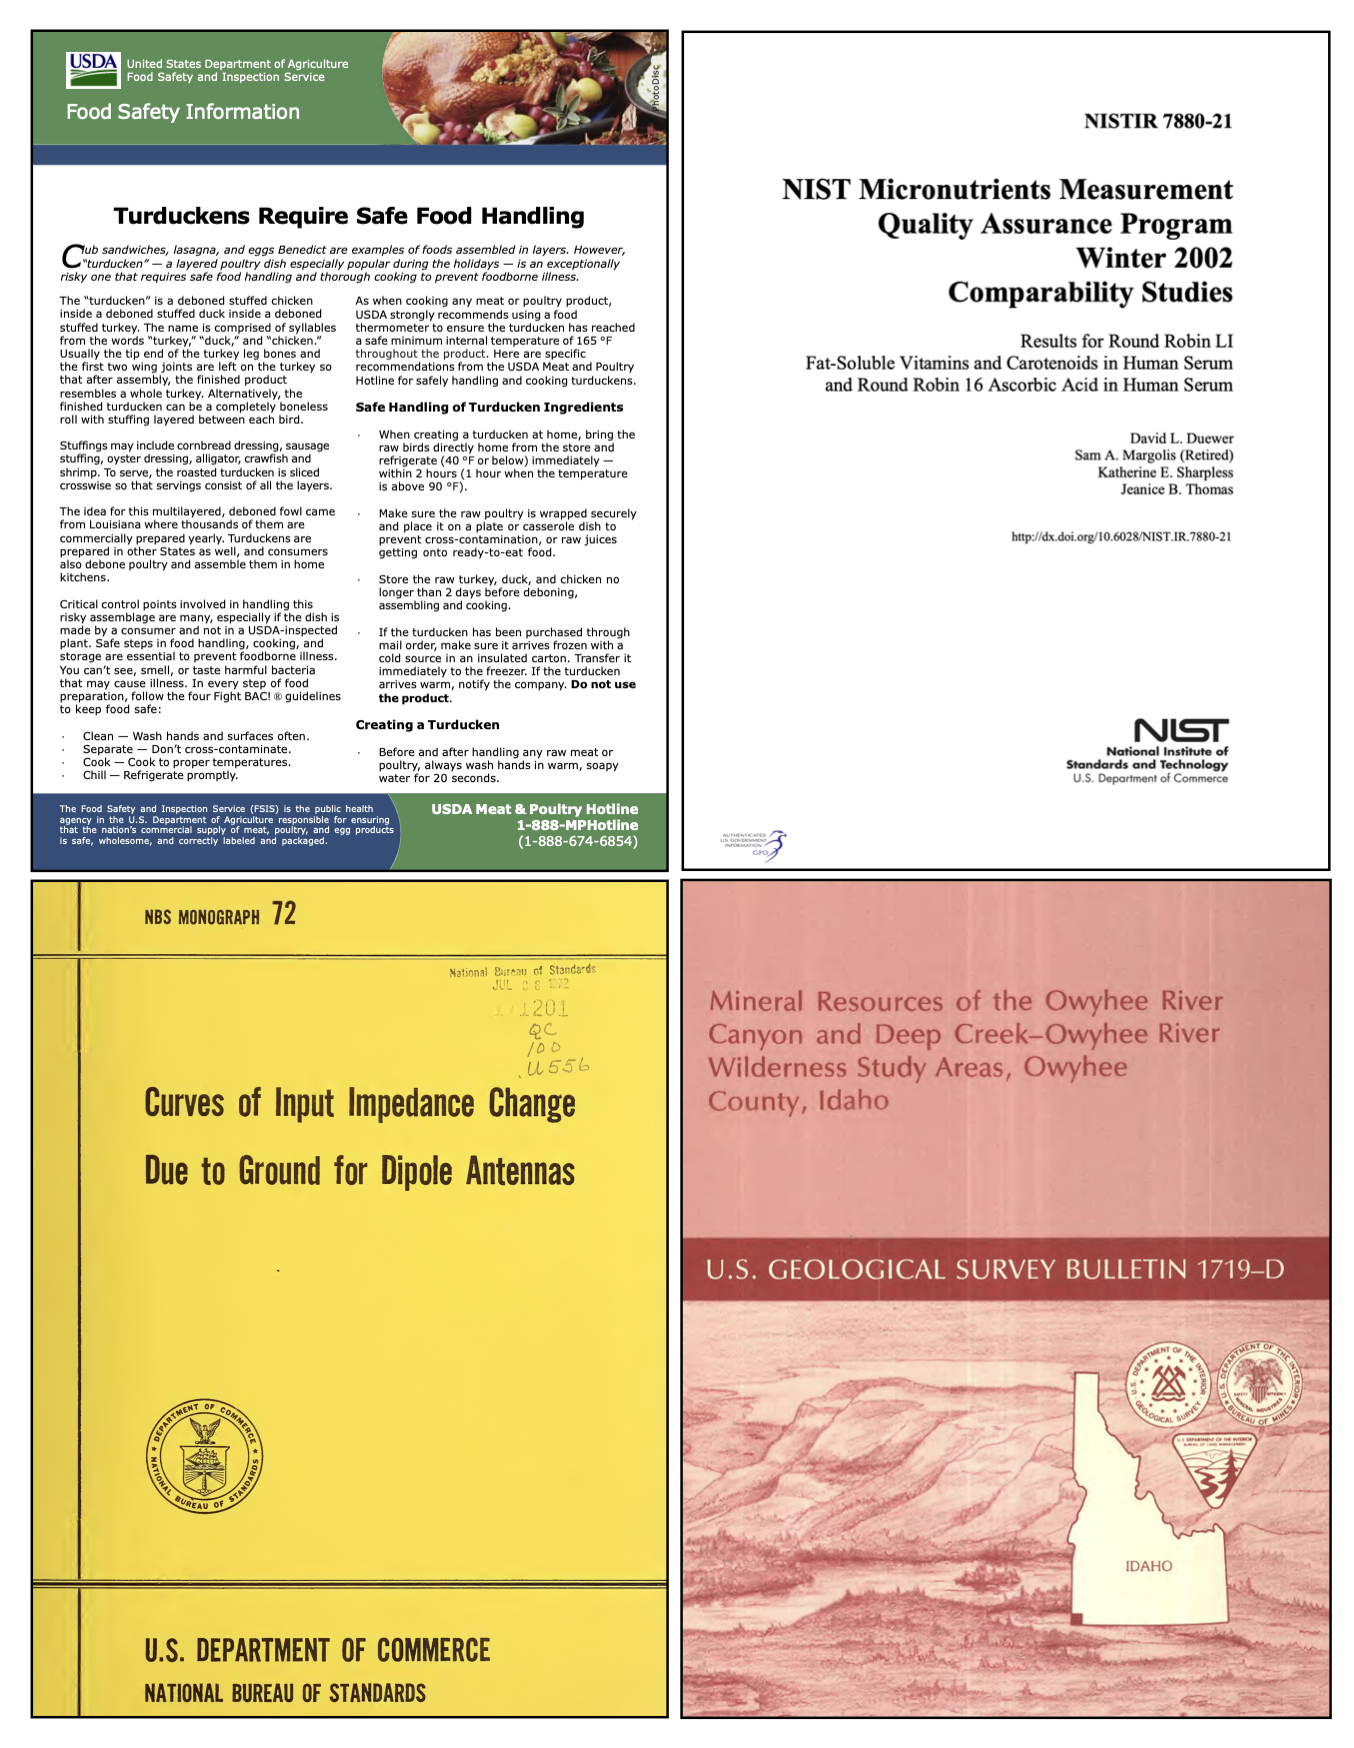
\includegraphics[width=95mm]{KL3MImages.png}
\caption{\centering{Samples of Content from the KL3M Dataset}}
\label{fig:KL3MImages}
\end{figure}

\subsection{The Collection \& Pre-Processing Data Pipeline for KL3M}
Working with the vast array of document types such as those displayed in Figure \ref{fig:KL3MImages} is a challenging proposition.  To do so effectively at scale, we developed a pre-processing pipeline designed to engage with the real-life challenges associated with the unstructured, inconsistent and complex forms of documents across the various information systems with which we engaged.  Thus, in addition to the KL3M dataset, we are also releasing all of the tooling and libraries leveraged across the KL3M Pre-Processing pipeline as it is our hope that others might adapt this work in order to build parallel corpora in other jurisdictions.   

\begin{figure}[h!]
\centering
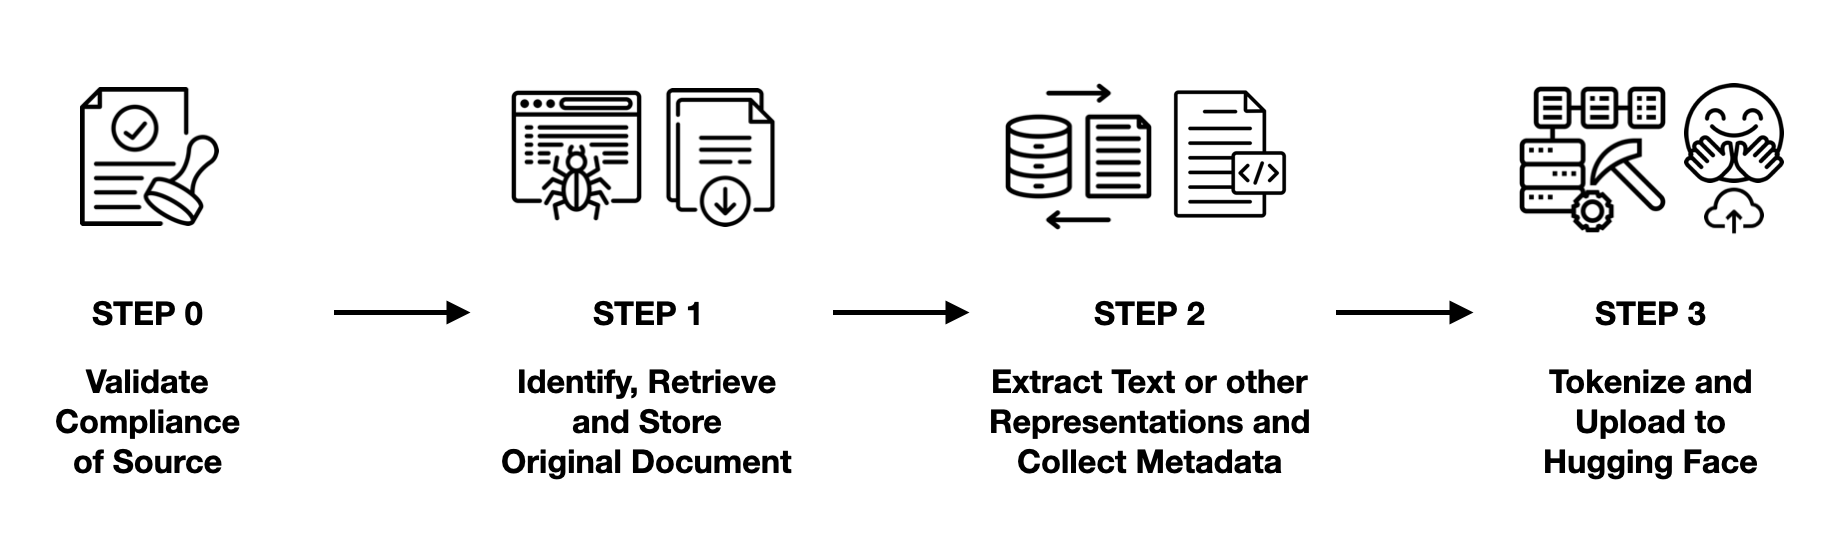
\includegraphics[width=150mm]{PreProcessing.png}
\caption{\centering{{Overview of the Pre-Processing Pipeline} - (icons via Flaticon)}}
\label{fig:preprocessing}
\end{figure}


Figure \ref{fig:preprocessing} provides a high-level overview of our pre-processing pipeline.  Building from our copyright filtration process described in Figure \ref{fig:CopyrightFlowchart}, we begin by identifying a potential source of useful content.  Next, we must determine whether that candidate source complies with our requirements. Thus, \textit{Step 0} is high level recitation of the process described in Figure \ref{fig:CopyrightFlowchart}.  Having then identified and validated compliance of the source material, we next proceed to \textit{Step 1} of Figure \ref{fig:preprocessing} where we retrieve and retain the original source material for provenance purposes.\footnote{This ability to demonstrate original source provenance was critical in obtaining the \textit{Fairly Trained} Certification described in Section 3.2.}  

In \textit{Step 2}, we develop an alternative representation of the documents which varies depending upon the nature of the original source.  Our ideal path is to build an alternative representation of all source materials in Markdown \cite{mailund2019beginner} while also retaining the original source material in parallel.  However, this is not always possible given the nature of the original source.  Finally, in \textit{Step 2} were also collect and store \textit{Dublin Core Metadata} for all source material.  

In \textit{Step 3}, we tokenize all objects using a custom tokenizer developed specifically for this task.  The KL3M tokenizer has several specific elements that makes it unique \color{red}\textbf{[MIKE ADD HERE 2-3 sentences]} \color{black}  Finally, we upload the tokenized document to their respective folder on \textit{Hugging Face}.\footnote{The KL3M Data can be access here \url{https://huggingface.co/collections/alea-institute/kl3m-data-679f9db9b6fd93f91c3c633e}}


%\section{Pre-Processing}
% Add details about the pre-processing steps applied to the data
\section{Dataset Characteristics}

\subsection{KL3M Components and Summary Statistics}
While currently limited mostly to governmental sources, the KL3M dataset features a relatively large and diverse set of content such as the content highlighted in Figure \ref{fig:KL3MImages}.  In Table \ref{table:summarystats}, we present summary statistics for the overall dataset.  In total, the KL3M dataset features more than 125 million documents, 1.7 trillion tokens and more than 80 terabyte of total information content.  

\begin{table}[!htbp]
    \small
    \centering
    \begin{tabularx}{0.6\linewidth}{X @{\hskip 3pt} l @{\hskip 3pt}}
        \toprule
        \textbf{KL3M Features} & \\
        \midrule
        Total Documents in KL3M & 126 Million Documents \\
        Total Tokens in KL3M  & 1.7 Trillion Tokens \\
        Total File Size & 80 Terabytes \\
        \midrule
        \bottomrule
    \end{tabularx}
    \caption{Summary Statistics for KL3M Dataset}
    \label{table:summarystats}
\end{table}

Given the range of sources as the vast interconnectedness of ideas, concepts, there is almost certainly duplicate content contained herein. A document may quote elements of other documents or otherwise incorporate concepts from other documents.  Thus, the overall token count is somewhat larger than if one were to consider something such as the total number unique n-gram combinations.  However, we did not deduplicate the underlying content as we envision a wide range of potential uses for this overall source material.  Downstream users can thus decide how to mix, match, segment or further pre-process the content in order to support their specific objective or use case.  

\begin{table}[!htbp]
   \footnotesize
  \centering 
    \begin{tabular*}{\linewidth}{Xlrrr|r}
    \toprule
    \textbf{KL3M Component}  & {\sc{File Size}} & {\sc Document Count} & {\sc Token Count} & {\sc Avg Token Per Doc}\\
    \midrule
    Securities \& Exchange Commission Filings & 00.0GiB & 0.0 & 0.0 & 0.0 \\
Congressional Documents & 00.0GiB & 0.0  & 0.0 & 0.0 \\
Congressional Bills & 00.0GiB & 0.0  & 0.0 & 0.0 \\
Code of Federal Regulations &  00.0GiB & 0.0 & 0.0 & 0.0 \\
Electronic Code of Federal Regulations &  00.0GiB & 0.0  & 0.0 & 0.0  \\
Federal Depository Library Program &  00.0GiB & 0.0 & 0.0 & 0.0  \\
Federal Register &  00.0GiB & 0.0  & 0.0 & 0.0 \\
Federal Judicial Center &  00.0GiB & 0.0 & 0.0 & 0.0  \\
CIA World Factbook &  00.0GiB & 0.0  & 0.0 & 0.0  \\
Congressional Research Service &  00.0GiB & 0.0 & 0.0 & 0.0 \\
United States Government Manual &  00.0GiB & 0.0 & 0.0 & 0.0 \\
Library of Congress - Country Profiles &  00.0GiB & 0.0 & 0.0 & 0.0 \\
Statutes at Large &  00.0GiB & 0.0  & 0.0 & 0.0 \\
Regulatory Submissions &  00.0GiB & 0.0 & 0.0 & 0.0 \\
United States Code &  00.0GiB & 0.0 & 0.0 & 0.0 \\
Court Documents - Opinions &  00.0GiB & 0.0 & 0.0 & 0.0 \\
Court Documents - Motions, Orders, etc. &  00.0GiB & 0.0 & 0.0 & 0.0\\
Court Documents - Dockets  &  00.0GiB & 0.0  & 0.0 & 0.0 \\
Black's Law Dictionary, 2nd Edition &  00.0GiB & 0.0 & 0.0 & 0.0 \\
U.S. Federal Government Websites &  00.0GiB & 0.0 & 0.0 & 0.0 \\
US Patent Grant Full Text Data &  00.0GiB & 0.0  & 0.0 & 0.0 \\
Official Journal of the European Union &  00.0GiB & 0.0 & 0.0 & 0.0 \\
    \midrule
    \textbf{Totals} & \textbf{0.0} & \textbf{0.0} & \textbf{0.0} & \textbf{0.0}   \\
    \bottomrule
    \end{tabular*}%
  \label{table:KL3M Components}%
      \caption{Summary Statistics of KL3M Components }
\end{table}

Table \ref{table:summarystats} displays the document counts, token counts and average tokens per document for each of the KL3M components.  While \textit{Securities \& Exchange Commission Filings} are the largest component of the dataset from a total documents and token perspective, there are some other large sources of input data.  Other large subset of data include [ FILL IN NEXT 3-4 items]  

Among some of the smaller KL3M components, there are interesting elements worthy of exploration including millions of conversational messages extracted from Congressional hearings, nearly 20 billion tokens worth of docket entiries 

Appendix II offers a more detailed description of each of the KL3M Components.  




\subsection{KL3M Additional Compositional Statistics}

\textbf{DISTRIBUTION OF DOCUMENT SIZE}

\begin{figure}[h!]
\centering
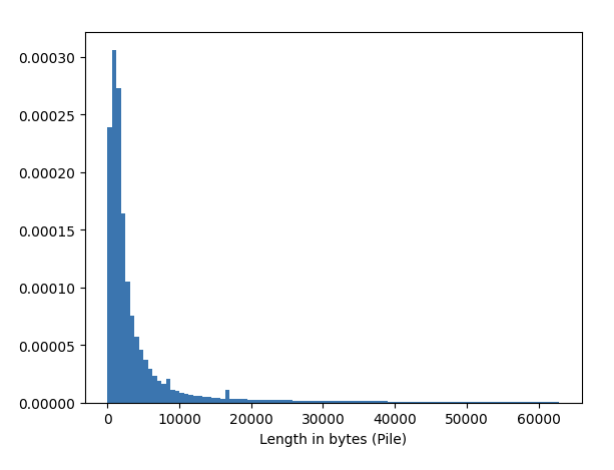
\includegraphics[width=90mm]{PileDist.png}
\caption{\centering{{Overview of the Pre-Processing Pipeline} - (icons via Flaticon)}}
\label{fig:Dist}
\end{figure}


\textbf{DISTRIBUTION OF PERPLEXITY SCORES}
\begin{figure}[h!]
\centering
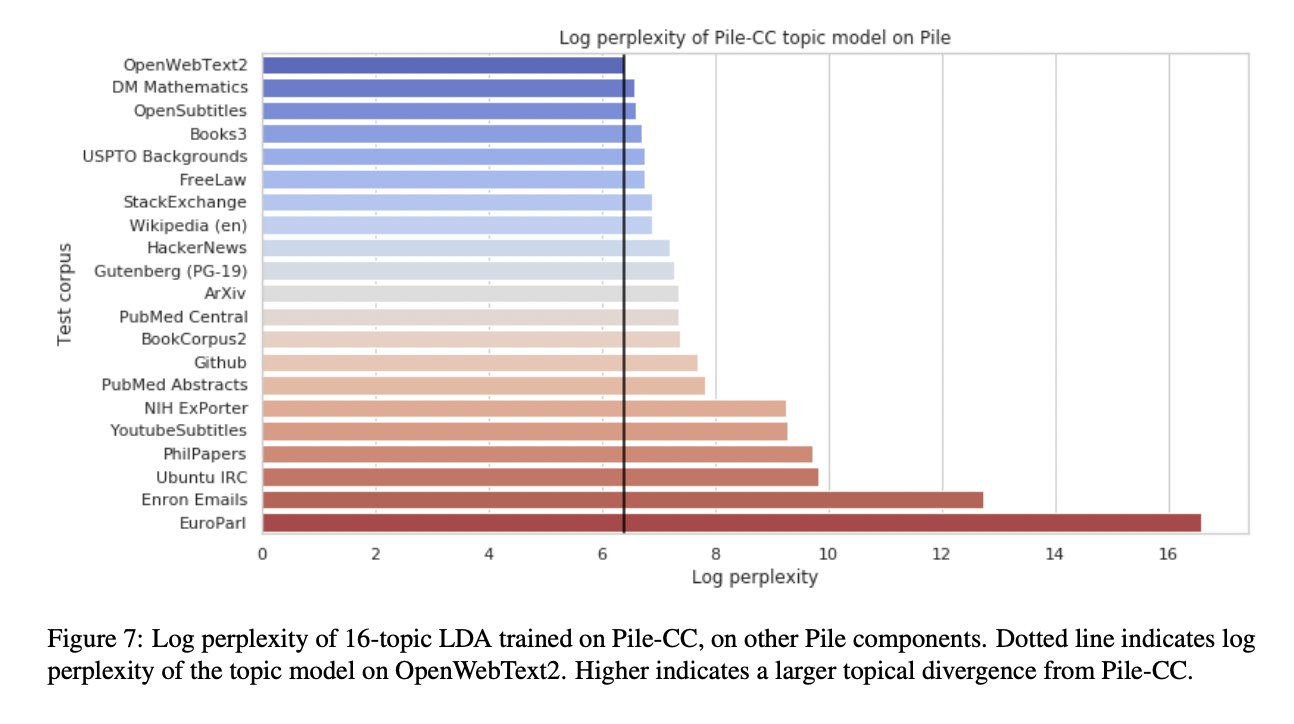
\includegraphics[width=110mm]{Perplexity.png}
\caption{\centering{{Overview of the Pre-Processing Pipeline} - (icons via Flaticon)}}
\label{fig:Perplexity}
\end{figure}


\textbf{TOXICITY ANALYSIS}
\begin{figure}[h!]
\centering
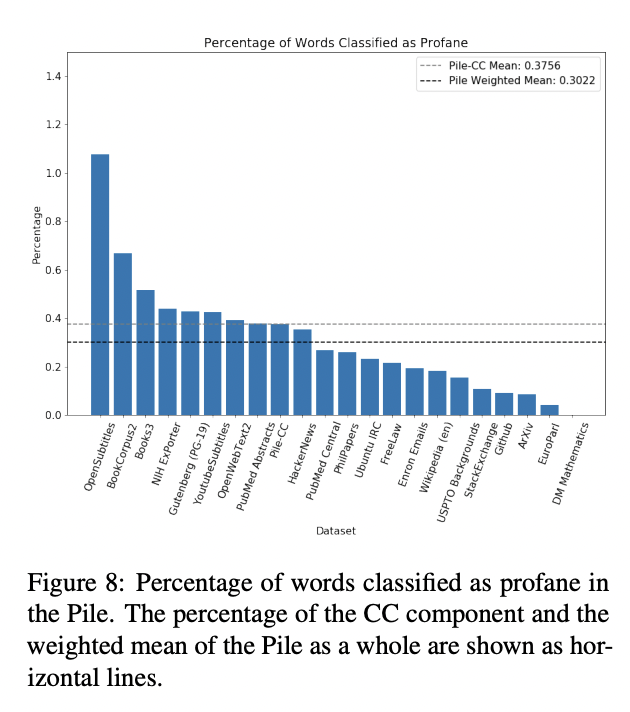
\includegraphics[width=90mm]{Toxicity.png}
\caption{\centering{{Overview of the Pre-Processing Pipeline} - (icons via Flaticon)}}
\label{fig:toxicity}
\end{figure}




Trying to copy some of the stuff reported in THE PILE paper 

\textbf{TOTAL TOKENS }

\vspace{10mm}

\textbf{TOTAL DOCS (with cavaet and discussion that doc is a tricky idea)}

\vspace{10mm}

\textbf{DISTRIBUTION OF TOKENS by Docs}

\vspace{10mm}

\textbf{SOME SORT OF TOKEN DIVERSITY MEASURE }

\vspace{10mm}





\textbf{Why US other countries -- data availability .. 
}





\section{A Living Dataset and Infrastructure for the Collecting and Distributing Copyright Clean Data}
In this paper, we introduced the Kelvin Legal Large Language Model (KL3M) dataset a large and diverse corpora of more than 125 million documents and more than 1.7 trillion tokens.  We describe our copyright filtration process designed to identify only source materials with clear provenance from a copyright perspective.  We then provided an overview of the pre-processing pipeline designed to 





The KL3M can be used in several ways.  First, it can serve as a baseline for model pretraining and could be combined with other appropriately license datasets.  Alternatively, it could be used to fine tune an existing model.  We realize that this dataset alone would likely be insufficent to allow for models to be built which cover the boundless set of possible use cases and user queries.  However, we believe this large body of tokens could be combined with selected forms of licensed content to develop LLMs which can deliver strong performance on certain tasks.  However, 
We believe that the development of datasets and models that are transparent, freely available without legal restrictions, and high quality will enable downstream use that is free of the infringement concerns often present.


The paper reflects the current version of the KL3M dataset as of the time of this publication.  Yet, rather than being a static snapshot, we hope that KL3M will persist as ``living dataset'' which we seek to update, maintain and extend as time moves forward.  In addition, we hope that KL3M will become a federated project where others leverage or retrofit some of our underlying infrastructure to expand the set of copyright clean data available from a global perspective.  

The KL3M dataset represents a significant step towards creating large language model training data that is free from copyright uncertainty. By carefully selecting and vetting our sources, we have created a resource that can be used with confidence by AI researchers and developers. We hope that our methodology will serve as a template for future efforts in this direction, ultimately leading to more legally and ethically robust AI systems.

As the field of AI continues to evolve rapidly, it is crucial that we address the legal and ethical challenges head-on. The KL3M dataset is our contribution to this effort, providing a foundation for the development of AI systems that can withstand future regulatory scrutiny and contribute positively to society.  While our focus has been on US and EU jurisdictions due to our familiarity with their legal systems, we recognize the need for similar efforts in other parts of the world. We encourage researchers and legal experts from other jurisdictions to adapt and expand upon our methodology to create globally representative datasets that are free from copyright concerns.

In conclusion, the KL3M dataset not only provides valuable training data for large language models but also sets a new standard for transparency and legal compliance in AI development. As we move forward, it is our hope that this work will inspire further innovation in the responsible and ethical advancement of AI technology.





\bibliographystyle{ieeetr}
\bibliography{article-min} 

\appendix
\section*{Appendices}
\addcontentsline{toc}{section}{Appendices}

\section{Caselaw Access Project (CAP)}
\label{appendix:cap}

This appendix provides details about the Caselaw Access Project (CAP) dataset, including its collection methodology, data statistics, and examples of the data. The Caselaw Access Project is a collaborative effort led by Harvard Law School's Library Innovation Lab to digitize and freely share all U.S. case law.

\subsection{Dataset Overview}

The CAP dataset contains court opinions from U.S. state and federal courts, providing a comprehensive repository of legal precedents. The corpus includes published opinions from all federal courts and state appellate courts, covering nearly 6.92 million cases from the 1700s to the present day. This represents one of the most comprehensive collections of historical and contemporary U.S. case law available for research and analysis.

\subsection{Data Processing Statistics}

Based on the counts files in the KL3M project, the CAP dataset has been processed through multiple stages:

\begin{table}[h]
\centering
\begin{tabular}{|l|r|}
\hline
\textbf{Processing Stage} & \textbf{Number of Documents} \\
\hline
Documents (Initial Collection) & 6,919,296 \\
Representations (Processed) & 6,919,272 \\
Parquet (Final Format) & 6,919,272 \\
\hline
\end{tabular}
\caption{CAP Dataset Document Counts by Processing Stage}
\label{tab:cap_counts}
\end{table}

As shown in Table \ref{tab:cap_counts}, nearly all collected documents (over 99.99\%) were successfully processed through each stage of the pipeline. The minimal difference between the initial collection count and the final processed count (24 documents) indicates the robustness of the processing pipeline for this dataset.

\subsection{Collection Methodology}

The CAP dataset was collected from the Harvard Law School's Case Law Access Project API and static archive. The collection process involved the following steps:

\begin{enumerate}
  \item A list of ZIP file URLs was compiled from the static.case.law archive, stored in the \texttt{zip\_urls.txt.gz} file within the KL3M codebase. Each URL points to a ZIP file containing multiple court opinions from a specific reporter.
  
  \item For each ZIP file URL, the collection pipeline:
  \begin{itemize}
    \item Downloads the ZIP archive from static.case.law
    \item Extracts both the HTML files (containing the case text) and the corresponding JSON metadata files
    \item Embeds each HTML fragment into a proper HTML document structure
    \item Creates a Document object with the following metadata:
    \begin{itemize}
      \item Unique ID from the CAP dataset
      \item Case name as the title
      \item Format identifier (text/html)
      \item Description (case name)
      \item Source URL (https://static.case.law/)
      \item License information (CC0 1.0 Universal)
      \item Content hash for integrity verification
      \item Case-specific metadata (court, jurisdiction, date, etc.)
    \end{itemize}
    \item Uploads each document to the KL3M storage system
  \end{itemize}
\end{enumerate}

The collection methodology leverages the publicly available data from the Case Law Access Project, which digitized over 40 million pages of U.S. court decisions in collaboration with Ravel Law. The dataset is licensed under CC0 1.0 Universal, placing it in the public domain. This ensures that the entire corpus is freely available for research, analysis, and reuse without copyright restrictions.

\subsection{Content Examples}
% TODO: Add representative examples of court opinions

\section{PACER Dockets}
\label{appendix:dockets}

This appendix provides details about the PACER Dockets dataset, including its collection methodology, data statistics, and examples of the data. PACER (Public Access to Court Electronic Records) is the electronic system that provides access to case and docket information from federal appellate, district, and bankruptcy courts.

\subsection{Dataset Overview}

The PACER Dockets dataset contains docket sheets from federal courts across the United States. These docket sheets serve as the official records of court proceedings, containing chronological listings of all events and filings in a case. The dataset includes dockets from district courts, bankruptcy courts, and appellate courts, providing a comprehensive record of federal court activity and procedural history.

The dockets provide essential metadata about federal cases, including:
\begin{itemize}
  \item Case numbers and titles
  \item Judge assignments
  \item Filing dates
  \item Party information (plaintiffs, defendants, attorneys)
  \item Chronological listing of all events and filings
  \item Case status and outcomes
\end{itemize}

\subsection{Data Processing Statistics}

Based on the counts files in the KL3M project, the PACER Dockets dataset has been processed through multiple stages:

\begin{table}[h]
\centering
\begin{tabular}{|l|r|}
\hline
\textbf{Processing Stage} & \textbf{Number of Documents} \\
\hline
Documents (Initial Collection) & 641,964 \\
Representations (Processed) & 641,961 \\
Parquet (Final Format) & 641,945 \\
\hline
\end{tabular}
\caption{PACER Dockets Dataset Document Counts by Processing Stage}
\label{tab:dockets_counts}
\end{table}

As shown in Table \ref{tab:dockets_counts}, the processing pipeline for the PACER Dockets dataset maintained high consistency across stages. From the initial collection to the representation stage, only 3 documents were lost (99.9995\% retention). The final parquet conversion stage had a minimal additional loss of 16 documents. Overall, 99.997\% of the originally collected documents were successfully processed through the entire pipeline, demonstrating the robustness of the processing methodology for this dataset.

\subsection{Collection Methodology}

The PACER Dockets dataset was collected from the CourtListener and Internet Archive's joint effort to make federal court records freely accessible. The collection process involved the following steps:

\begin{enumerate}
  \item Obtaining the source data file: The dataset retrieves a compressed CSV file (\texttt{dockets-2024-08-31.csv.bz2}) from the CourtListener's S3 storage bucket (\texttt{com-courtlistener-storage}). This file contains metadata about hundreds of thousands of federal docket sheets.
  
  \item Filtering and processing records: The source code filters the data to include only records with valid Internet Archive JSON URLs (records containing a \texttt{filepath\_ia\_json} field with a valid HTTP URL). Each record in the CSV contains extensive metadata about a court case, including:
  \begin{itemize}
    \item Court identifiers (e.g., \texttt{flnd} for Florida Northern District)
    \item Case numbers and PACER case IDs
    \item Case names (e.g., \texttt{Salvador v. Morgan})
    \item Filing and termination dates
    \item Nature of suit and cause of action
    \item Judge assignments
    \item Jurisdiction information
  \end{itemize}
  
  \item Downloading and processing JSON data: For each valid record, the system:
  \begin{itemize}
    \item Downloads the complete docket sheet in JSON format from the Internet Archive URL
    \item Creates a document record with the docket data
    \item Assigns a unique ID based on the JSON filename
    \item Preserves all original metadata in the document's \texttt{extra} field
    \item Calculates a cryptographic hash (blake2b) of the content for integrity verification
    \item Uploads the document to the KL3M storage system
  \end{itemize}
\end{enumerate}

The collection methodology leverages public domain federal court records made accessible through CourtListener and the Internet Archive. As noted in the source code, these docket entries are "Not subject to copyright under 17 U.S.C. 105 and provided under CC0 by CourtListener/IA." This status ensures that the entire dataset is freely available for research and analysis without copyright restrictions.

The dataset specifically focuses on the docket sheets themselves, which provide the procedural history and metadata of cases, rather than the full text of court documents (which are collected separately in the RECAP Documents dataset).

\subsection{Content Examples}
% TODO: Add representative examples of docket entries

\section{Federal Websites}
\label{appendix:dotgov}

This appendix provides details about the Federal Websites dataset, which contains content from U.S. government websites in the .gov, .mil, and select other government-related domains. These websites represent official information from various federal agencies, departments, and institutions across all branches of government.

\subsection{Processing Statistics}

Table~\ref{table:dotgov-stats} shows the processing statistics for the Federal Websites dataset.

\begin{table}[h]
\centering
\begin{tabular}{|l|r|r|r|}
\hline
\textbf{Processing Stage} & \textbf{Document Count} & \textbf{\% of Documents} & \textbf{\% of Initial} \\
\hline
Documents (Initial Collection) & 3,233,136 & 100\% & 100\% \\
Representations (Processed) & 3,191,427 & 98.7\% & 98.7\% \\
Parquet (Final Format) & 3,187,567 & 98.6\% & 98.6\% \\
\hline
\end{tabular}
\caption{Processing statistics for the Federal Websites dataset.}
\label{table:dotgov-stats}
\end{table}

The Federal Websites dataset demonstrates an excellent processing success rate of 98.6\% from initial collection to final format. This high rate indicates the quality and accessibility of government web content, with only minimal data loss during processing. The slight reduction between the Representations and Parquet stages (only 3,860 documents) further demonstrates the stability of the dataset through the processing pipeline.

\subsection{Domain Coverage}

The KL3M dataset includes content from hundreds of federal websites across multiple government branches and agencies. These domains can be organized into several major categories:

\begin{itemize}
  \item \textbf{Executive Branch Agencies} -- Includes websites from cabinet departments (e.g., www.dhs.gov, www.treasury.gov), independent agencies (e.g., www.epa.gov, www.nasa.gov), and their sub-agencies
  \item \textbf{Legislative Branch} -- Includes www.house.gov, www.senate.gov, www.gao.gov, www.cbo.gov
  \item \textbf{Judicial Branch} -- Includes court websites such as www.uscourts.gov and circuit courts
  \item \textbf{Military Domains} -- Various .mil domains including www.army.mil, www.navy.mil, www.af.mil
\end{itemize}

This broad coverage ensures representation from across the U.S. federal government, capturing the diversity of information produced by different agencies and institutions.

\subsection{Collection Methodology}

The Federal Websites dataset is collected through a comprehensive approach designed to capture diverse content types while filtering out non-informative materials. The collection methodology involves:

\begin{enumerate}
    \item \textbf{Source Selection} -- Carefully selecting government domains from the .gov and .mil TLDs, focusing on federal agencies
    
    \item \textbf{Content Filtering} -- Implementing sophisticated file type filtering that:
    \begin{itemize}
        \item Includes informative document formats like HTML, PDF, Word documents, Excel spreadsheets, PowerPoint presentations, XML, and plain text
        \item Excludes non-informative formats like images (PNG, JPG, GIF), style files (CSS), scripts (JS), and multimedia (MP3, MP4)
        \item Applies size thresholds to ensure document quality
    \end{itemize}
    
    \item \textbf{Metadata Extraction} -- For each document:
    \begin{itemize}
        \item Extracting basic metadata like title and description from HTML meta tags
        \item For PDFs, extracting embedded metadata and page counts using PyPDFium2
        \item Computing cryptographic hashes (blake2b) for content integrity verification
    \end{itemize}
    
    \item \textbf{Legal Compliance} -- Ensuring adherence to the public domain status of federal government works under 17 U.S.C. § 105, while filtering content that might have copyright restrictions
\end{enumerate}

This methodical approach ensures comprehensive coverage of valuable government information while maintaining data quality and legal compliance.

\subsection{Document Types and Content}

The Federal Websites dataset encompasses a wide variety of document types reflecting the diverse nature of government communications:

\begin{enumerate}
    \item \textbf{Web Pages (HTML/XHTML)}
    \begin{itemize}
        \item Agency information pages describing missions, services, and operations
        \item Public guidance and instructions for government services
        \item Press releases and news announcements
        \item Reports and publications in web format
    \end{itemize}
    
    \item \textbf{Document Files}
    \begin{itemize}
        \item PDFs of reports, studies, guidelines, and forms
        \item Word documents (.doc, .docx) with detailed information
        \item Spreadsheets (.xls, .xlsx) containing data and statistics
        \item Presentations (.ppt, .pptx) from government briefings
    \end{itemize}
    
    \item \textbf{Data Formats}
    \begin{itemize}
        \item XML files containing structured data
        \item CSV files with tabular data
        \item RSS and Atom feeds providing updates from agencies
    \end{itemize}
\end{enumerate}

The dataset specifically excludes non-informative content such as images, style sheets, scripts, and multimedia files to focus on textual and structured information.

\subsection{Technical Implementation}

The Federal Websites dataset collection is implemented using Python with several key technical components:

\begin{enumerate}
    \item \textbf{Content Type Detection}
    \begin{itemize}
        \item Using the \texttt{mimetypes} library to identify file types
        \item Implementing fallback mechanisms for ambiguous content types
        \item Maintaining allowlists (INCLUDE\_MIME\_TYPES) and blocklists (EXCLUDE\_EXTENSIONS) to filter content
    \end{itemize}
    
    \item \textbf{Metadata Extraction}
    \begin{itemize}
        \item Using regular expressions (HTML\_TITLE\_RE, HTML\_META\_RE) to extract HTML metadata
        \item Leveraging PyPDFium2 for PDF parsing and metadata extraction
        \item Normalizing inconsistent metadata fields (e.g., title vs. Title)
    \end{itemize}
    
    \item \textbf{Document Processing}
    \begin{itemize}
        \item Managing document identifiers based on source domain and path
        \item Handling various character encodings and format peculiarities
        \item Implementing error handling for malformed documents
    \end{itemize}
\end{enumerate}

This robust implementation ensures efficient processing of diverse government content while maintaining high data quality standards.

\subsection{Legal Status}

The Federal Websites dataset is primarily in the public domain under 17 U.S.C. § 105, which specifies that works created by the U.S. federal government are not subject to copyright protection. As stated in the dataset metadata: "Public domain under 17 U.S. Code § 105 after filtering copyrighted material and excluded agencies/GSEs."

The collection process includes filtering to exclude:

\begin{enumerate}
    \item Content from government-sponsored enterprises (GSEs) which may not be subject to the same public domain provisions
    \item Third-party copyrighted material that might be embedded in government websites
    \item Material from agencies explicitly excluded from the public domain provisions
\end{enumerate}

This careful filtering ensures the dataset's compliance with copyright law while maximizing the availability of valuable government information.

\subsection{Research Applications}

The Federal Websites dataset offers numerous research opportunities:

\begin{enumerate}
    \item \textbf{Government Operations Analysis}
    \begin{itemize}
        \item Studying how agencies communicate with the public
        \item Analyzing policy implementation across different agencies
        \item Tracking changes in government priorities over time
    \end{itemize}
    
    \item \textbf{Natural Language Processing}
    \begin{itemize}
        \item Training models on official government language and terminology
        \item Developing information extraction tools for government documents
        \item Creating summarization systems for lengthy government reports
    \end{itemize}
    
    \item \textbf{Public Information Studies}
    \begin{itemize}
        \item Measuring accessibility and readability of government communications
        \item Analyzing consistency of information across agencies
        \item Studying public data disclosure practices
    \end{itemize}
    
    \item \textbf{Digital Government Research}
    \begin{itemize}
        \item Evaluating e-government implementations
        \item Studying digital service delivery models
        \item Analyzing government website usability and information architecture
    \end{itemize}
\end{enumerate}

The dataset's comprehensive coverage of federal web content makes it valuable for researchers across multiple disciplines interested in government operations, communication, and information dissemination.
\section{Electronic Code of Federal Regulations (eCFR)}
\label{appendix:ecfr}

This appendix provides details about the Electronic Code of Federal Regulations (eCFR) dataset, including its collection methodology, data statistics, and examples of the data. The eCFR is a web version of the Code of Federal Regulations (CFR) that is maintained by the U.S. Government Publishing Office (GPO) and updated daily to better reflect its current status.

\subsection{Dataset Overview}

The eCFR dataset contains the full text of all federal regulations organized into 50 titles, covering broad subject areas of federal regulation. The dataset provides a complete, up-to-date version of the U.S. Code of Federal Regulations, including all active regulations from federal agencies. This dataset is particularly valuable as it represents the official codification of the general and permanent rules published in the Federal Register by the executive departments and agencies of the Federal Government.

\subsection{Data Processing Statistics}

Based on the counts files in the KL3M project, the eCFR dataset has been processed through multiple stages:

\begin{table}[h]
\centering
\begin{tabular}{|l|r|}
\hline
\textbf{Processing Stage} & \textbf{Number of Documents} \\
\hline
Documents (Initial Collection) & 262,243 \\
Representations (Processed) & 262,243 \\
Parquet (Final Format) & 262,243 \\
\hline
\end{tabular}
\caption{eCFR Dataset Document Counts by Processing Stage}
\label{tab:ecfr_counts}
\end{table}

As shown in Table \ref{tab:ecfr_counts}, the eCFR dataset maintained perfect consistency across all processing stages, with 100\% of documents successfully preserved through the entire pipeline. This demonstrates the exceptional quality and robustness of both the source data and the processing methodology for this dataset.

\subsection{Collection Methodology}

The eCFR dataset was collected using the official eCFR API provided by the U.S. Government Publishing Office. The collection process involved the following steps:

\begin{enumerate}
  \item \textbf{Title Retrieval}: The system first retrieved metadata about all 50 CFR titles using the \verb|/api/versioner/v1/titles.json| endpoint.
  
  \item \textbf{Version Discovery}: For each title, the system obtained the latest available version date using the \verb|/api/versioner/v1/versions/title-{title}.json| endpoint.
  
  \item \textbf{Structure Mapping}: For each title as of its latest version date, the system retrieved the complete hierarchical structure using the \verb|/api/versioner/v1/structure/{date}/title-{title}.json| endpoint. This structure contains all levels of the regulatory hierarchy, including:
  \begin{itemize}
    \item Titles (e.g., Title 1: General Provisions)
    \item Chapters (e.g., Chapter I: Office of the Federal Register)
    \item Subchapters (when applicable)
    \item Parts (e.g., Part 1: Federal Register)
    \item Subparts (when applicable)
    \item Sections (e.g., §1.1 Definitions)
  \end{itemize}
  
  \item \textbf{Section Content Retrieval}: The system then traversed each title's structure to identify all section nodes, which represent the actual regulatory content. For each section, it retrieved the HTML content using the \verb|/api/renderer/v1/content/enhanced/{date}/title-{title}?section={section}| endpoint.
  
  \item \textbf{Document Creation}: For each section, a Document object was created with comprehensive metadata:
  \begin{itemize}
    \item Unique ID in the format \verb|{date}/{title}/{section}|
    \item Title from the section label
    \item Description combining the title, section, and date information
    \item HTML content of the regulation
    \item Publisher information (U.S. Government Publishing Office)
    \item Date of the regulation version
    \item Cryptographic hash (blake2b) for integrity verification
  \end{itemize}
  
  \item \textbf{Storage}: Each document was uploaded to the KL3M storage system.
\end{enumerate}

The collection process incorporates a rate-limiting mechanism (with a delay of 0.1 seconds between requests) to ensure compliance with the eCFR API's usage policies and to avoid overwhelming the government servers.

\subsection{Legal Status}

As noted in the source code, the eCFR dataset is "Not subject to copyright under 17 U.S.C. 105," which means that the content is in the public domain as it was created by the federal government. This makes the dataset freely available for research, analysis, and redistribution without copyright restrictions.

\subsection{Content Structure}

The eCFR content is structured hierarchically, following the official organization of the Code of Federal Regulations:

\begin{itemize}
  \item \textbf{Titles} (1-50): Broad subject areas (e.g., Title 10 - Energy, Title 26 - Internal Revenue)
  \item \textbf{Chapters}: Typically corresponding to the issuing agency
  \item \textbf{Subchapters}: Further divisions within chapters (when applicable)
  \item \textbf{Parts}: Major topical divisions within chapters or subchapters
  \item \textbf{Subparts}: Divisions within parts (when applicable)
  \item \textbf{Sections}: The basic unit of the CFR, containing the actual regulatory text
  \item \textbf{Appendices}: Supplementary material to parts or sections
\end{itemize}

This hierarchical structure is preserved in the KL3M dataset, allowing for comprehensive coverage and navigation of the entire federal regulatory framework.

\section{SEC EDGAR Database}
\label{appendix:edgar}

This appendix provides details about the SEC EDGAR Database dataset, including its collection methodology, data statistics, and examples of the data. The Electronic Data Gathering, Analysis, and Retrieval (EDGAR) system is the primary system for companies and individuals to submit required forms and documents to the U.S. Securities and Exchange Commission (SEC).

\subsection{Dataset Overview}

The EDGAR dataset contains corporate filings submitted to the U.S. Securities and Exchange Commission (SEC) under various securities laws including the Securities Act of 1933, the Securities Exchange Act of 1934, the Trust Indenture Act of 1939, and the Investment Company Act of 1940. These filings include annual reports (10-K), quarterly reports (10-Q), registration statements, prospectuses, proxy statements, and various other corporate disclosures required by federal securities laws.

The dataset provides a comprehensive repository of public company disclosures dating back to 1996, serving as a critical resource for financial research, regulatory compliance analysis, and corporate transparency studies. The EDGAR archive is particularly valuable as it contains standardized corporate financial information across thousands of public companies over multiple decades.

\subsection{Data Processing Statistics}

Based on the counts files in the KL3M project, the EDGAR dataset has been processed through multiple stages:

\begin{table}[h]
\centering
\begin{tabular}{|l|r|}
\hline
\textbf{Processing Stage} & \textbf{Number of Documents} \\
\hline
Documents (Initial Collection) & 74,063,501 \\
Representations (Processed) & 30,474,244 \\
Parquet (Final Format) & 44,768,118 \\
\hline
\end{tabular}
\caption{EDGAR Dataset Document Counts by Processing Stage}
\label{tab:edgar_counts}
\end{table}

As shown in Table \ref{tab:edgar_counts}, the EDGAR dataset exhibits some interesting patterns through the processing pipeline. The initial collection contained over 74 million documents, of which approximately 41\% were successfully converted to representations. However, the parquet format shows a higher document count than the representations stage, suggesting that some documents may have been processed through alternative pipelines or that the parquet conversion included additional fields or transformations that resulted in multiple parquet files per original document.

The large difference between the initial document count and the representations count likely reflects the complex nature of EDGAR filings, which often contain multiple document types, some of which may be difficult to process (like certain PDF formats, image-based documents, or proprietary formats) or may have been intentionally filtered during processing.

\subsection{Collection Methodology}

The EDGAR dataset was collected directly from the SEC's EDGAR system using their public API. The collection process involved several sophisticated steps:

\begin{enumerate}
  \item \textbf{Daily Feed Collection}: The system downloads daily feed files from the SEC EDGAR archives, going back to 1996 (specified by the \texttt{EDGAR\_MIN\_DATE} constant). Each feed is a tar.gz archive containing multiple "nc" (News Condensed) files.
  
  \item \textbf{Feed Processing}: For each daily feed archive, the system:
  \begin{itemize}
    \item Extracts all member files from the tar.gz archive
    \item Processes each .nc file containing multiple submissions
  \end{itemize}
  
  \item \textbf{Submission Parsing}: Within each .nc file, the system:
  \begin{itemize}
    \item Identifies submission blocks using regex pattern matching
    \item Extracts metadata from the submission header
    \item Identifies individual document blocks within each submission
  \end{itemize}
  
  \item \textbf{Document Extraction}: For each document in a submission:
  \begin{itemize}
    \item Extracts document metadata (type, sequence, filename, description)
    \item Extracts the document content from between \texttt{<TEXT>} tags
    \item Handles UUEncoded content by decoding when necessary
  \end{itemize}
  
  \item \textbf{Document Creation}: For each extracted document, a Document object is created with extensive metadata:
  \begin{itemize}
    \item Unique ID in the format \texttt{cik/accession\_number/sequence}
    \item URL to the document on the SEC website
    \item Document content and size
    \item Content hash for integrity verification
    \item MIME type based on file extension
    \item Document title from the description field
    \item Source name from filer/issuer/subject company information
    \item SEC as the publisher
    \item Filing date
    \item Form types as subjects
    \item Complete submission and document metadata in the extra field
  \end{itemize}
  
  \item \textbf{Storage}: Each document is uploaded to the KL3M storage system.
\end{enumerate}

The collection process includes extensive error handling to manage the variations in document formats and metadata structures found in the EDGAR archive. It also carefully maintains the SEC-specific metadata hierarchy, preserving the relationships between companies, submissions, and documents.

\subsection{Legal Status}

As noted in the source code, the EDGAR dataset is "Generally accepted to available for free use and distribution" under various securities laws including Sections 19 and 20 of the Securities Act of 1933, Section 21 of the Securities Exchange Act of 1934, Section 321 of the Trust Indenture Act of 1939, Section 42 of the Investment Company Act of 1940, Section 209 of the Investment Advisers Act of 1940, and Title 17 of the Code of Federal Regulations, Section 202.5.

The code does note the ISDA v. Socratek case as offering some potentially countervailing guidance, but the general understanding is that these materials are not subject to copyright and are available for public use as records of the U.S. government.

\subsection{Content Types}

The EDGAR dataset includes a wide variety of document types, reflecting the diverse nature of corporate filings:

\begin{itemize}
  \item \textbf{Annual Reports (10-K, 10-KSB)} - Comprehensive reports on a company's financial performance
  \item \textbf{Quarterly Reports (10-Q, 10-QSB)} - Updates on a company's financial status for a fiscal quarter
  \item \textbf{Registration Statements (S-1, S-3, etc.)} - Filings for new security offerings
  \item \textbf{Beneficial Ownership Reports (Schedule 13D, 13G)} - Reports of ownership of more than 5\% of a company
  \item \textbf{Insider Trading Reports (Form 3, 4, 5)} - Reports of insider transactions
  \item \textbf{Proxy Statements (DEF 14A)} - Information provided to shareholders before annual meetings
  \item \textbf{Current Reports (8-K)} - Reports of significant events between regular filings
  \item \textbf{Foreign Company Reports (20-F, 40-F)} - Annual reports for foreign companies
\end{itemize}

The dataset preserves both the structured metadata about these filings and the full content of the documents themselves, enabling comprehensive analysis of corporate disclosures across time and across different regulatory requirements.

\section{European Union Official Journal}
\label{appendix:eu_oj}

This appendix provides details about the European Union Official Journal dataset, including its collection methodology, data statistics, and examples of the data.

% TODO: Add specific details about this dataset

\section{Federal Depository Library Program}
\label{appendix:fdlp}

This appendix provides details about the Federal Depository Library Program dataset, including its collection methodology, data statistics, and examples of the data.

% TODO: Add specific details about this dataset

\section{Federal Register}
\label{appendix:fr}

This appendix provides details about the Federal Register dataset, including its collection methodology, data statistics, and examples of the data. The Federal Register is the official journal of the United States government, containing federal agency regulations, proposed rules, public notices, executive orders, proclamations, and other presidential documents.

\subsection{Dataset Overview}

The Federal Register dataset contains the complete collection of documents published in the Federal Register since 1995. It serves as the official source for federal regulations, notices, and presidential documents, making it essential for legal research, regulatory compliance, and policy analysis. The dataset provides access to the full text of proposed rules, final rules, notices, and presidential documents published daily by Federal agencies.

This dataset is particularly valuable because it represents the official publication through which regulatory changes are announced, public comments are solicited, and new federal requirements are established. It covers all executive branch agencies and provides a comprehensive record of the federal regulatory process.

\subsection{Data Processing Statistics}

Based on the counts files in the KL3M project, the Federal Register dataset has been processed through multiple stages:

\begin{table}[h]
\centering
\begin{tabular}{|l|r|}
\hline
\textbf{Processing Stage} & \textbf{Number of Documents} \\
\hline
Documents (Initial Collection) & 3,396,818 \\
Representations (Processed) & 3,396,455 \\
Parquet (Final Format) & 3,396,389 \\
\hline
\end{tabular}
\caption{Federal Register Dataset Document Counts by Processing Stage}
\label{tab:fr_counts}
\end{table}

As shown in Table \ref{tab:fr_counts}, the Federal Register dataset maintained exceptional consistency across all processing stages. From the initial collection to the representation stage, only 363 documents were lost (99.99\% retention). The final parquet conversion stage had a minimal additional loss of 66 documents. Overall, 99.99\% of the originally collected documents were successfully processed through the entire pipeline, demonstrating the high quality of both the source data and the processing methodology.

\subsection{Collection Methodology}

The Federal Register dataset was collected using the official Federal Register API provided by the Government Publishing Office (GPO) and the National Archives and Records Administration (NARA). The collection process involved several sophisticated steps:

\begin{enumerate}
  \item \textbf{Date-Based Retrieval}: The system iterates through all dates from January 1, 1995 (\texttt{FR\_MIN\_DATE}) to the present day, retrieving all documents published on each date.
  
  \item \textbf{Document Discovery}: For each date, the system queries the Federal Register API (\texttt{/api/v1/documents.json}) with a comprehensive set of metadata fields to identify all documents published on that date.
  
  \item \textbf{Multiple Format Collection}: For each document identified, the system retrieves all available formats:
  \begin{itemize}
    \item \textbf{XML}: Full XML content from the \texttt{full\_text\_xml\_url} endpoint, providing structured data about the document
    \item \textbf{Plain Text}: Raw text content from the \texttt{raw\_text\_url} endpoint
    \item \textbf{PDF}: PDF version from the \texttt{pdf\_url} endpoint
    \item \textbf{HTML}: HTML content from the \texttt{body\_html\_url} endpoint, which includes the formatted document
  \end{itemize}
  
  \item \textbf{Document Creation}: For each format of each document, the system creates a Document object with comprehensive metadata:
  \begin{itemize}
    \item Unique ID in the format \texttt{document\_number/extension}
    \item Document content in the specific format
    \item Size and cryptographic hash (blake2b) for integrity verification
    \item Title and abstract from the original document
    \item Publication date
    \item Agency information as creator metadata
    \item Subject information from document type, subtype, and topics
    \item Citation and bibliographic information
    \item Complete metadata from the API response in the extra field
  \end{itemize}
  
  \item \textbf{Storage}: Each format of each document is uploaded to the KL3M storage system.
\end{enumerate}

The collection process includes sophisticated error handling to ensure that even if retrieval of one format fails, other formats can still be processed and stored. It also applies rate limiting to respect the API's usage policies and avoid overwhelming the government servers.

\subsection{Document Types}

The Federal Register contains several distinct types of documents, each serving a different purpose in the federal regulatory process:

\begin{itemize}
  \item \textbf{Proposed Rules}: Documents announcing draft regulations and soliciting public comments
  \item \textbf{Rules}: Final regulations with the force of law
  \item \textbf{Notices}: Announcements of meetings, information collections, grant applications, etc.
  \item \textbf{Presidential Documents}: Executive orders, proclamations, and other presidential actions
  \item \textbf{Sunshine Act Meetings}: Announcements of federal agency meetings open to the public
  \item \textbf{Corrections}: Documents correcting errors in previously published materials
\end{itemize}

\subsection{Legal Status}

As noted in the source code, the Federal Register dataset is "Not subject to copyright under 17 U.S.C. 105," which means that the content is in the public domain as it was created by the federal government. This makes the dataset freely available for research, analysis, and redistribution without copyright restrictions.

\subsection{Data Transformation}

The collection process includes the capability to transform XML documents using an XSLT stylesheet (\texttt{fedregister.xsl}). This transformation converts the structured XML content into HTML format, preserving the document's structure while making it more accessible for viewing and analysis. The XSLT transformation carefully preserves elements such as:

\begin{itemize}
  \item Document headers and metadata
  \item Agency and action information
  \item CFR references and regulatory text
  \item Structural elements like sections, paragraphs, and tables
  \item Formatting for special elements like footnotes, appendices, and signatures
\end{itemize}

This transformation ensures that the rich structure of Federal Register documents is maintained while being made accessible in standard web formats.

\section{GovInfo}
\label{appendix:govinfo}

This appendix provides details about the GovInfo dataset, which contains official publications from all three branches of the Federal Government. GovInfo is a service of the United States Government Publishing Office (GPO), providing free public access to a comprehensive repository of government information.

\subsection{Processing Statistics}

Table~\ref{table:govinfo-stats} shows the processing statistics for the GovInfo dataset.

\begin{table}[h]
\centering
\begin{tabular}{|l|r|r|r|}
\hline
\textbf{Processing Stage} & \textbf{Document Count} & \textbf{\% of Documents} & \textbf{\% of Initial} \\
\hline
Documents (Initial Collection) & 14,655,232 & 100\% & 100\% \\
Representations (Processed) & 13,353,022 & 91.1\% & 91.1\% \\
Parquet (Final Format) & 11,144,653 & 76.0\% & 76.0\% \\
\hline
\end{tabular}
\caption{Processing statistics for the GovInfo dataset.}
\label{table:govinfo-stats}
\end{table}

The GovInfo dataset shows a good initial processing success rate of 91.1\% from raw documents to representations, with some additional reduction to 76.0\% in the final parquet stage. This processing pattern reflects the diverse nature of government publications, which include complex document formats, nested structures, and varying content quality. The dataset still maintains over 11 million documents in the final format, making it one of the largest components of the KL3M collection.

\subsection{Collections}

The KL3M dataset includes content from multiple collections available in GovInfo. Some documents may appear in multiple collections, as indicated by the semicolon-delimited collection IDs in the source data. The primary collections are:

\begin{itemize}
  \item \textbf{BILLS} -- Congressional Bills
  \item \textbf{BUDGET} -- Budget of the United States Government
  \item \textbf{CCAL} -- Congressional Calendars
  \item \textbf{CDIR} -- Congressional Directory
  \item \textbf{CDOC} -- Congressional Documents
  \item \textbf{CHRG} -- Congressional Hearings
  \item \textbf{CMR} -- Commerce Business Daily
  \item \textbf{COMPS} -- Compilations of Presidential Documents
  \item \textbf{CPD} -- Congressional Pictorial Directory
  \item \textbf{CPRT} -- Congressional Committee Prints
  \item \textbf{CREC} -- Congressional Record
  \item \textbf{CRECB} -- Congressional Record Bound
  \item \textbf{CRI} -- Congressional Record Index
  \item \textbf{CRPT} -- Congressional Reports
  \item \textbf{CZIC} -- Coastal Zone Information Center
  \item \textbf{ECONI} -- Economic Indicators
  \item \textbf{ERIC} -- Education Resources Information Center
  \item \textbf{ERP} -- Economic Report of the President
  \item \textbf{GAOREPORTS} -- Government Accountability Office Reports
  \item \textbf{GOVMAN} -- Government Manual
  \item \textbf{GOVPUB} -- Government Publications
  \item \textbf{GPO} -- Government Publishing Office Collections
  \item \textbf{HJOURNAL} -- House Journal
  \item \textbf{HMAN} -- House Manual
  \item \textbf{HOB} -- History of Bills
  \item \textbf{LSA} -- List of CFR Sections Affected
  \item \textbf{PAI} -- Privacy Act Issuances
  \item \textbf{PLAW} -- Public and Private Laws
  \item \textbf{PPP} -- Public Papers of the Presidents
  \item \textbf{SERIALSET} -- Serial Set
  \item \textbf{SMAN} -- Senate Manual
  \item \textbf{SJOURNAL} -- Senate Journal
  \item \textbf{STATUTE} -- Statutes at Large
  \item \textbf{USCOURTS} -- United States Courts Opinions
\end{itemize}

\subsection{Cross-Collection Documents}

Some documents in GovInfo appear in multiple collections. The major cross-collection occurrences include:

\begin{itemize}
  \item Documents that appear in both their primary collection and the GPO collection (e.g., documents labeled as GPO;CDOC, GPO;CFR, GPO;CPRT, GPO;CRECB, GPO;CRPT, GPO;FR, GPO;SJOURNAL)
  \item Documents in the Serial Set that also belong to other collections (e.g., SERIALSET;CDOC, SERIALSET;CRPT, SERIALSET;HJOURNAL, SERIALSET;SJOURNAL)
  \item Congressional documents that appear in multiple collections (e.g., ERP;CDOC, HMAN;CDOC, SMAN;CDOC)
  \item Government publications in specific categories (e.g., GOVPUB;CHRG)
  \item Budget documents in multiple collections (SERIALSET;CDOC;BUDGET)
  \item Economic reports in multiple collections (SERIALSET;CRPT;ERP)
\end{itemize}

\subsection{Collection Methodology}

The GovInfo dataset is collected through the official GovInfo API provided by the U.S. Government Publishing Office. The collection methodology involves:

\begin{enumerate}
    \item \textbf{API Integration} -- Using the official GovInfo API with authenticated access through an API key
    
    \item \textbf{Systematic Collection} -- Retrieving documents through several complementary approaches:
    \begin{itemize}
        \item Collection-based retrieval targeting specific government collections
        \item Date-based retrieval covering documents from 1995 to the present
        \item Granule-level retrieval for collections with nested document structures
    \end{itemize}
    
    \item \textbf{Metadata Extraction} -- For each document:
    \begin{itemize}
        \item Retrieving comprehensive metadata including title, date issued, collection code, and government author
        \item Processing multi-collection documents to ensure proper categorization
        \item Handling temporal relationships between documents
    \end{itemize}
    
    \item \textbf{Content Download} -- Implementing a sophisticated download process that:
    \begin{itemize}
        \item Prioritizes text and PDF formats over ZIP archives when available
        \item Handles the on-demand generation of package content through API retry mechanisms
        \item Processes both package-level and granule-level content
    \end{itemize}
    
    \item \textbf{Duplicate Avoidance} -- Excluding collections already covered by separate specialized datasets (specifically CFR and FR)
\end{enumerate}

The collection process includes robust error handling for service interruptions, rate limiting compliance, and handling of dynamically generated content. The system implements intelligent caching to optimize API usage and ensure comprehensive coverage.

\subsection{Document Structure and Content Types}

The GovInfo dataset encompasses a diverse range of document types and formats reflecting the variety of government publications:

\begin{enumerate}
    \item \textbf{Document Organization}
    \begin{itemize}
        \item \textit{Packages} -- Top-level container for related documents
        \item \textit{Granules} -- Subdivisions within packages (e.g., sections of a bill, chapters of a report)
        \item \textit{Collections} -- Thematic groupings of documents by government function or source
    \end{itemize}
    
    \item \textbf{Content Formats}
    \begin{itemize}
        \item PDF documents for formatted reading
        \item Text formats for plain text content
        \item HTML/XML for structured online viewing
        \item ZIP archives containing multiple related documents
    \end{itemize}
    
    \item \textbf{Content Categories}
    \begin{itemize}
        \item Legislative materials (bills, reports, hearings)
        \item Executive publications (presidential papers, agency reports)
        \item Judicial documents (court opinions)
        \item Administrative documents (manuals, directories)
    \end{itemize}
\end{enumerate}

The system prioritizes the most accessible and useful formats, preferring text and PDF formats when available to ensure optimal processing in the KL3M pipeline.

\subsection{Metadata and Search Capabilities}

The GovInfo collection leverages rich metadata available through the API:

\begin{enumerate}
    \item \textbf{Identification Information}
    \begin{itemize}
        \item Package ID and Granule ID for unique document identification
        \item Collection codes indicating document source and category
        \item Document class distinguishing document types
    \end{itemize}
    
    \item \textbf{Temporal Information}
    \begin{itemize}
        \item Date issued for official publication date
        \item Last modified date for tracking updates
        \item Date ingested into the GovInfo system
    \end{itemize}
    
    \item \textbf{Legislative Context}
    \begin{itemize}
        \item Congress number for legislative session
        \item Session identifier for specific congressional period
        \item Branch indicator (Executive, Legislative, Judicial)
    \end{itemize}
    
    \item \textbf{Content Description}
    \begin{itemize}
        \item Title providing document summary
        \item Category classifying content type
        \item Government author attributing the creating entity
    \end{itemize}
\end{enumerate}

This rich metadata enables complex searches and filtering capabilities, allowing targeted retrieval based on various criteria including date ranges, government branches, document types, and content categories.

\subsection{Legal Status}

The GovInfo dataset is primarily in the public domain under 17 U.S.C. § 105, which states that works created by the federal government are not subject to copyright protection. As specified in the dataset metadata: "In general, GovInfo documents fall under 17 U.S.C. 101 and 17 U.S.C. 105 and are therefore not subject to copyright protection. Any incorporated material not covered by these provisions will be clearly marked with a notice per 17 U.S.C. 403."

The legal status ensures that:

\begin{enumerate}
    \item Government-produced content is freely available for research and analysis
    \item Third-party content incorporated into government documents is properly identified with copyright notices as required by law
    \item The dataset can be used without copyright restrictions for a wide range of applications
\end{enumerate}

\subsection{Research Applications}

The GovInfo dataset offers numerous research opportunities:

\begin{enumerate}
    \item \textbf{Legislative Analysis}
    \begin{itemize}
        \item Tracking the evolution of bills through Congress
        \item Analyzing voting patterns and legislative priorities
        \item Studying the language and structure of federal legislation
    \end{itemize}
    
    \item \textbf{Government Operations}
    \begin{itemize}
        \item Examining congressional hearing transcripts for policy development
        \item Analyzing budget documents for fiscal priorities
        \item Studying government reports for agency activities and recommendations
    \end{itemize}
    
    \item \textbf{Legal Research}
    \begin{itemize}
        \item Analyzing court opinions for legal precedents
        \item Studying the implementation of statutes and regulations
        \item Tracking changes in legal interpretation over time
    \end{itemize}
    
    \item \textbf{Political Science}
    \begin{itemize}
        \item Analyzing presidential communications and policy statements
        \item Studying congressional deliberations and debates
        \item Examining the relationship between branches of government
    \end{itemize}
\end{enumerate}

The comprehensive nature of this dataset, spanning all three branches of government, makes it particularly valuable for researchers interested in U.S. governance, policy development, and legal analysis.
\section{RECAP Archive}
\label{appendix:recap}

This appendix provides details about the RECAP Archive dataset, which consists of documents and filings from the federal judiciary's Public Access to Court Electronic Records (PACER) system that have been collected by the Free Law Project's RECAP initiative.

\subsection{Processing Statistics}

Table \ref{table:recap-stats} shows the processing statistics for the RECAP Archive dataset.

\begin{table}[h]
\centering
\begin{tabular}{|l|r|r|r|}
\hline
\textbf{Processing Stage} & \textbf{Document Count} & \textbf{\% of Documents} & \textbf{\% of Initial} \\
\hline
Documents (Initial Collection) & 16,762,471 & 100\% & 100\% \\
Representations (Processed) & 14,423,347 & 86.0\% & 86.0\% \\
Parquet (Final Format) & 14,265,800 & 85.1\% & 85.1\% \\
\hline
\end{tabular}
\caption{Processing statistics for the RECAP Archive dataset.}
\label{table:recap-stats}
\end{table}

\subsection{Collection Methodology}

The RECAP Archive dataset is collected from the Free Law Project's RECAP initiative, which allows users of the PACER system to contribute documents they have accessed to a public archive. The collection methodology involves:

\begin{enumerate}
    \item Accessing the public Court Listener S3 bucket (com-courtlistener-storage) where the RECAP project stores the contributed documents.
    \item Iterating through all objects with the prefix "recap/" in the S3 bucket.
    \item Processing each document, extracting metadata, and deduplicating based on content hashes (using blake2b).
    \item For PDF files, extracting additional metadata using the pypdfium2 library, including page count and embedded document metadata.
    \item For XML files (specifically docket XML files), extracting basic metadata.
    \item Storing the documents with appropriate metadata including court information, document type, and source attribution.
\end{enumerate}

The collection process includes court identification, which maps court identifiers (e.g., "ca1", "nysd") to their full names (e.g., "United States Court of Appeals for the First Circuit", "United States District Court for the Southern District of New York").

\subsection{Document Types}

The RECAP Archive dataset includes two primary document types:

\begin{enumerate}
    \item \textbf{PDF documents} - These include various court filings such as complaints, motions, orders, opinions, and other legal documents that are filed in federal courts. The PDFs are processed to extract metadata such as page count, title, author, and other embedded information.
    
    \item \textbf{XML docket files} - These files, ending with ".docket.xml", contain structured information about court cases, including case metadata, party information, and a chronological list of docket entries describing the documents filed in the case.
\end{enumerate}

Both document types provide valuable information about federal court cases, with the PDF files containing the actual text of legal documents and the XML files providing structured case data.

\subsection{Legal Status}

The RECAP Archive dataset is made available under CC0/Public Domain. While federal court documents are generally considered public domain under 17 U.S.C. § 105, which excludes works of the U.S. Government from copyright protection, the PACER system itself charges access fees. The RECAP project makes these public domain documents freely available by collecting them from users who have already paid for access.

According to the Free Law Project, "court opinions are not copyrightable and thus remain in the public domain. Court orders and other documents created by courts as part of their official duties are also not copyrightable." Documents submitted by parties in court cases may potentially be subject to copyright, though they are considered publicly accessible once filed in court.

\subsection{Distinguishing RECAP Archive from RECAP Documents}

It's important to note the distinction between the "recap" dataset described in this section and the related "recap\_docs" dataset (covered in the next section). The main differences are:

\begin{enumerate}
    \item The RECAP Archive ("recap") contains primarily docket entries and main case documents retrieved from PACER.
    \item The RECAP Documents ("recap\_docs") contains attachment files associated with court documents, including various file formats like .doc, .docx, .mp3, .pdf, and .wpd.
\end{enumerate}

Together, these datasets provide a comprehensive view of federal court cases and filings.
\section{RECAP Documents}
\label{appendix:recap_docs}

This appendix provides details about the RECAP Documents dataset, which consists of document attachments from the federal judiciary's Public Access to Court Electronic Records (PACER) system collected by the Free Law Project's RECAP initiative. Unlike the main RECAP Archive (Section~\ref{appendix:recap}), which focuses on dockets and main filing documents, this dataset specifically contains file attachments in various formats.

\subsection{Processing Statistics}

Table~\ref{table:recap-docs-stats} shows the processing statistics for the RECAP Documents dataset.

\begin{table}[h]
\centering
\begin{tabular}{|l|r|r|r|}
\hline
\textbf{Processing Stage} & \textbf{Document Count} & \textbf{\% of Documents} & \textbf{\% of Initial} \\
\hline
Documents (Initial Collection) & 1,863,733 & 100\% & 100\% \\
Representations (Processed) & 1,691,658 & 90.8\% & 90.8\% \\
Parquet (Final Format) & 1,691,655 & 90.8\% & 90.8\% \\
\hline
\end{tabular}
\caption{Processing statistics for the RECAP Documents dataset.}
\label{table:recap-docs-stats}
\end{table}

The RECAP Documents dataset shows a high processing success rate of 90.8\%, with only a minimal loss between the Representations and Parquet stages (only 3 documents). This indicates that most of the document attachments in various formats were successfully processed through the entire pipeline.

\subsection{Collection Methodology}

The RECAP Documents dataset is collected using a specialized data source class (\texttt{RECAPDocSource}) that interacts with the Free Law Project's public S3 storage. The collection methodology involves:

\begin{enumerate}
    \item Accessing the public Court Listener S3 bucket (\texttt{com-courtlistener-storage}) where RECAP documents are stored.
    \item Iterating through objects in five specific prefix directories that represent different file formats:
    \begin{itemize}
        \item \texttt{doc/} - Microsoft Word documents
        \item \texttt{docx/} - Microsoft Word Open XML documents
        \item \texttt{mp3/} - Audio files
        \item \texttt{pdf/} - PDF documents
        \item \texttt{wpd/} - WordPerfect documents
    \end{itemize}
    \item Processing each document through the following steps:
    \begin{itemize}
        \item Checking if the document already exists in the collection to avoid duplication
        \item Fetching the document content from the S3 bucket
        \item Computing a blake2b hash of the document content for deduplication
        \item Determining the appropriate MIME type based on the file extension
        \item Creating a Document object with metadata including dataset ID, identifier, size, hash, format, source, and publisher
        \item Storing the document in the KL3M collection
    \end{itemize}
\end{enumerate}

Unlike the main RECAP Archive, which contains detailed court information and specific metadata extraction for PDF files, the RECAP Documents source focuses on preserving a wide variety of file formats with their original content. The collection process handles different file types appropriately by determining their MIME types and creating a standardized metadata structure.

\subsection{Document Types and Content}

The RECAP Documents dataset contains various file formats commonly used in legal proceedings:

\begin{enumerate}
    \item \textbf{Microsoft Word documents} (.doc, .docx)
    \begin{itemize}
        \item Legal briefs and memoranda
        \item Written declarations and affidavits
        \item Expert reports and analyses
        \item Contractual documents and agreements
        \item Correspondence submitted as evidence
    \end{itemize}
    
    \item \textbf{PDF documents} (.pdf)
    \begin{itemize}
        \item Scanned exhibits and evidence
        \item Technical reports and studies
        \item Business records
        \item Published articles submitted as references
        \item Charts, graphs, and other visual evidence
    \end{itemize}
    
    \item \textbf{Audio files} (.mp3)
    \begin{itemize}
        \item Recorded depositions
        \item Hearing transcripts in audio format
        \item Recorded phone conversations submitted as evidence
        \item Audio evidence relevant to cases
    \end{itemize}
    
    \item \textbf{WordPerfect documents} (.wpd)
    \begin{itemize}
        \item Legacy legal documents from courts or attorneys still using WordPerfect
        \item Older filings that maintain their original format
    \end{itemize}
\end{enumerate}

The wide variety of document formats makes this dataset particularly valuable for understanding the full scope of materials presented in federal court cases. Unlike many text-centric legal datasets, RECAP Documents captures the multimedia nature of modern legal proceedings.

\subsection{Legal Status}

The RECAP Documents dataset is made available under CC0/Public Domain designation. While court documents themselves are generally considered public domain under 17 U.S.C. § 105, it's important to note that:

\begin{enumerate}
    \item Attachments submitted by private parties may potentially contain copyrighted material
    \item Once filed with a court, these documents become part of the public record and are accessible through PACER
    \item The RECAP project's mission is to make these publicly accessible documents freely available without the access fees charged by the PACER system
\end{enumerate}

The Free Law Project, which maintains the RECAP Archive, asserts that "documents filed in federal courts are, with very few exceptions, in the public domain or available via fair use." However, researchers should be aware that some embedded third-party content within documents may have different copyright status than the court documents themselves.

\subsection{Technical Implementation}

The RECAP Documents collection is implemented using Python with the following key technical components:

\begin{enumerate}
    \item \texttt{hashlib.blake2b} for cryptographic hashing and deduplication
    \item \texttt{mimetypes} library for determining appropriate MIME types
    \item AWS S3 API for accessing the Court Listener storage bucket
    \item Custom document processing pipeline that handles various file formats
\end{enumerate}

The collection code includes robust error handling to manage issues like network failures, corrupt files, or missing content. It also implements a tracking system to avoid duplicate documents across the collection process.

\subsection{Relationship to Other Datasets}

The RECAP Documents dataset complements several other datasets in the KL3M collection:

\begin{enumerate}
    \item \textbf{RECAP Archive} (Section~\ref{appendix:recap}) - Contains the main dockets and primary filing documents, while RECAP Documents contains the attachments and exhibits referenced in those filings
    \item \textbf{Court Listener} (Section~\ref{appendix:cap}) - Focuses on court opinions, while RECAP Documents contains the supporting materials that may have informed those opinions
    \item \textbf{Dockets} (Section~\ref{appendix:dockets}) - Contains structured information about case proceedings, while RECAP Documents provides the actual content of exhibits and attachments
\end{enumerate}

When used together, these datasets provide a comprehensive view of the U.S. federal court system, from procedural information to substantive legal arguments and supporting evidence.

\subsection{Research Applications}

The RECAP Documents dataset is particularly valuable for:

\begin{enumerate}
    \item \textbf{Legal research} requiring access to the full context of cases, including exhibits and supporting materials
    \item \textbf{Natural language processing} tasks across multiple document formats in the legal domain
    \item \textbf{Multi-modal analysis} of legal proceedings, including text, scanned documents, and audio
    \item \textbf{Studies of evidence types} used in different categories of federal litigation
    \item \textbf{Legal education} providing realistic examples of legal document preparation
\end{enumerate}

The dataset's inclusion of various file formats makes it particularly valuable for researchers interested in developing tools that can process the heterogeneous document types encountered in legal practice.
\section{Regulations.gov Documents}
\label{appendix:reg_docs}

This appendix provides details about the Regulations.gov Documents dataset, which consists of documents submitted to the federal rulemaking portal, including public comments, proposed rules, supporting materials, and regulatory attachments.

\subsection{Processing Statistics}

Table~\ref{table:reg-docs-stats} shows the processing statistics for the Regulations.gov Documents dataset.

\begin{table}[h]
\centering
\begin{tabular}{|l|r|r|r|}
\hline
\textbf{Processing Stage} & \textbf{Document Count} & \textbf{\% of Documents} & \textbf{\% of Initial} \\
\hline
Documents (Initial Collection) & 1,279,349 & 100\% & 100\% \\
Representations (Processed) & 811,163 & 63.4\% & 63.4\% \\
Parquet (Final Format) & 785,062 & 61.4\% & 61.4\% \\
\hline
\end{tabular}
\caption{Processing statistics for the Regulations.gov Documents dataset.}
\label{table:reg-docs-stats}
\end{table}

The Regulations.gov Documents dataset shows a processing success rate of 61.4\% from initial collection to final format. This relatively lower conversion rate compared to some other datasets in the KL3M collection is likely due to the diverse nature of submitted documents, which include various file formats, scanned images, and occasionally corrupted files submitted through the public comment system.

\subsection{Collection Methodology}

The Regulations.gov Documents dataset is collected using the official Regulations.gov API v4. The collection methodology involves:

\begin{enumerate}
    \item Accessing the Regulations.gov API using an API key (required for all operations)
    \item Systematically retrieving documents by date, starting from January 1, 2010
    \item For each date, retrieving all documents posted on that date using pagination to handle large result sets
    \item For each document, retrieving detailed information including all associated file formats and attachments
    \item Downloading the content of each document and attachment from the provided file URLs
    \item Processing each document through the following steps:
    \begin{itemize}
        \item Checking if the document already exists in the collection to avoid duplication
        \item Determining the document's content type from response headers
        \item Extracting metadata such as title, posted date, and agency ID
        \item Generating a blake2b hash of the document content
        \item Creating a Document object with comprehensive metadata
        \item Storing the document in the KL3M collection
    \end{itemize}
\end{enumerate}

The collection process includes sophisticated rate limiting techniques to comply with API restrictions. The system dynamically adjusts request delays based on the rate limit information provided in API response headers, increasing or decreasing delays to optimize throughput while avoiding API rate limit errors.

\subsection{API Details and Rate Limiting}

The Regulations.gov API v4 enforces strict rate limits on requests. To manage these limits, the collection process:

\begin{enumerate}
    \item Tracks the number of remaining API requests through response headers
    \item Implements adaptive delay between requests:
    \begin{itemize}
        \item Decreases delay by 2.5\% when rate limit headroom increases
        \item Increases delay by 5\% when rate limit headroom decreases
        \item Maintains a slight decrease (0.5\%) when usage remains stable
        \item Enforces minimum and maximum delay bounds (2.0-6.5 seconds)
    \end{itemize}
    \item Handles API errors and temporary failures with appropriate retries
\end{enumerate}

This adaptive approach ensures efficient collection while maintaining compliance with the API's terms of service.

\subsection{Document Types and Content}

The Regulations.gov Documents dataset encompasses a wide variety of document types related to the federal rulemaking process:

\begin{enumerate}
    \item \textbf{Public Comments}
    \begin{itemize}
        \item Feedback from individuals, organizations, and stakeholders on proposed regulations
        \item Personal statements, expert opinions, and grassroots responses
        \item Form letters and mass comment campaigns
    \end{itemize}
    
    \item \textbf{Supporting Materials}
    \begin{itemize}
        \item Scientific studies and research papers
        \item Technical analyses and impact assessments
        \item Economic evaluations and cost-benefit analyses
        \item Market surveys and industry data
    \end{itemize}
    
    \item \textbf{Attachments and Exhibits}
    \begin{itemize}
        \item Data tables, charts, and graphs
        \item Photographs and diagrams
        \item Engineering specifications and technical drawings
        \item Affidavits and witness statements
    \end{itemize}
    
    \item \textbf{Regulatory Documents}
    \begin{itemize}
        \item Proposed rules and regulatory text
        \item Supplementary information and background materials
        \item Response to comments documents
        \item Regulatory flexibility analyses
    \end{itemize}
\end{enumerate}

Documents are primarily stored in PDF format, though the original submission may have been in various formats. The Regulations.gov system typically converts uploads to PDF for consistent public access.

\subsection{Metadata Structure}

Each document in the dataset contains rich metadata including:

\begin{enumerate}
    \item \textbf{Basic Identifiers}
    \begin{itemize}
        \item Document ID (e.g., EPA-HQ-OPP-2007-1024-0726)
        \item Unique identifier URL (e.g., https://downloads.regulations.gov/EPA-HQ-OPP-2007-1024-0726/content.pdf)
    \end{itemize}
    
    \item \textbf{Temporal Information}
    \begin{itemize}
        \item Posted date (when the document was made available on Regulations.gov)
    \end{itemize}
    
    \item \textbf{Authorship and Publishing Details}
    \begin{itemize}
        \item Agency ID (the federal agency responsible for the regulatory action)
        \item Document title
        \item Content type (usually application/pdf)
    \end{itemize}
    
    \item \textbf{Technical Metadata}
    \begin{itemize}
        \item Content size in bytes
        \item Cryptographic hash (blake2b) for integrity verification
        \item Original API response containing full document details
    \end{itemize}
\end{enumerate}

The dataset preserves all original metadata from the Regulations.gov API, enabling researchers to access the complete context of each document.

\subsection{Legal Status}

The Regulations.gov Documents dataset is made available according to the Regulations.gov User Notice, which permits unrestricted third-party use of the materials. Key aspects of the legal status include:

\begin{enumerate}
    \item Public domain status for documents created by federal agencies (under 17 U.S.C. § 105)
    \item Public records status for submitted comments and materials
    \item Attribution to the eRulemaking Program Management Office as the publisher
    \item Attribution to the specific federal agency as the creator for agency-produced documents
\end{enumerate}

While the documents themselves are freely available for use, researchers should be aware that some submitted materials might contain third-party content with different copyright status.

\subsection{Research Value}

The Regulations.gov Documents dataset offers unique research opportunities:

\begin{enumerate}
    \item \textbf{Regulatory Process Analysis}
    \begin{itemize}
        \item Understanding public participation in rulemaking
        \item Studying the evolution of regulatory text based on public input
        \item Analyzing the quality and impact of public comments
    \end{itemize}
    
    \item \textbf{Natural Language Processing Applications}
    \begin{itemize}
        \item Sentiment analysis of public comments
        \item Topic modeling of regulatory discussions
        \item Extraction of technical arguments and evidence
        \item Classification of comment types and stakeholder groups
    \end{itemize}
    
    \item \textbf{Policy Impact Studies}
    \begin{itemize}
        \item Measuring public response to proposed regulations
        \item Identifying key concerns across different regulatory domains
        \item Tracking changes in regulatory approach over time
    \end{itemize}
\end{enumerate}

The dataset provides a comprehensive view of public participation in the U.S. federal regulatory process, capturing diverse viewpoints from individuals, businesses, non-profits, and other stakeholders.

\subsection{Relationship to Other Datasets}

The Regulations.gov Documents dataset complements other regulatory datasets in the KL3M collection:

\begin{enumerate}
    \item \textbf{Federal Register} (Section~\ref{appendix:fr}) - Contains the official published proposed and final rules, while Regulations.gov Documents contains the public comments and supporting materials
    
    \item \textbf{Electronic Code of Federal Regulations} (Section~\ref{appendix:ecfr}) - Represents the final codified regulations, while Regulations.gov Documents shows the development process and public input
    
    \item \textbf{GovInfo} (Section~\ref{appendix:govinfo}) - Provides broader government publications, while Regulations.gov Documents focuses specifically on regulatory development materials
\end{enumerate}

Together, these datasets provide a comprehensive view of the U.S. regulatory landscape, from initial proposal through public comment to final implementation.
\section{UK Legislation}
\label{appendix:ukleg}

This appendix provides details about the UK Legislation dataset, including its collection methodology, data statistics, and examples of the data. The UK Legislation dataset consists of primary and secondary legislation from the United Kingdom, published on the legislation.gov.uk website maintained by The National Archives.

\subsection{Processing Statistics}

Table~\ref{table:ukleg-stats} shows the processing statistics for the UK Legislation dataset.

\begin{table}[h]
\centering
\begin{tabular}{|l|r|r|r|}
\hline
\textbf{Processing Stage} & \textbf{Document Count} & \textbf{\% of Documents} & \textbf{\% of Initial} \\
\hline
Documents (Initial Collection) & 219,190 & 100\% & 100\% \\
Representations (Processed) & 219,190 & 100\% & 100\% \\
Parquet (Final Format) & 219,190 & 100\% & 100\% \\
\hline
\end{tabular}
\caption{Processing statistics for the UK Legislation dataset.}
\label{table:ukleg-stats}
\end{table}

The UK Legislation dataset shows a perfect 100\% processing success rate across all stages. This exceptional conversion rate indicates the high quality and consistency of the source data, which is provided in a standardized HTML format that processes extremely well through the KL3M pipeline.

\subsection{Dataset Coverage}

The dataset includes various types of UK legislation:

\begin{itemize}
  \item \textbf{Acts of Parliament} -- Primary legislation enacted by the UK Parliament
  \item \textbf{Statutory Instruments} -- Secondary legislation made under powers delegated by Acts of Parliament
  \item \textbf{Statutory Rules and Orders} -- Historical statutory instruments predating 1948
  \item \textbf{UK Statutory Rules} -- Northern Ireland statutory rules
  \item \textbf{UK Church Instruments} -- Measures and instruments related to the Church of England
  \item \textbf{UK Local Acts} -- Acts that apply to specific localities or entities rather than the general public
\end{itemize}

The dataset covers legislation dating back to 1267, with comprehensive coverage of legislation enacted after 1988. Older legislation is added to the dataset as it is digitized by The National Archives.

\subsection{Collection Methodology}

The UK Legislation dataset is collected from the official legislation.gov.uk archive, which is maintained by The National Archives of the UK. The collection methodology involves:

\begin{enumerate}
    \item Accessing the public bulk data package provided by The National Archives, specifically the "revised-all-versions-html.zip" archive available at \texttt{http://leggovuk-ldn.s3-website.eu-west-2.amazonaws.com/texts/revised-all-versions/html/}
    
    \item Processing each HTML file in the archive through the following steps:
    \begin{itemize}
        \item Checking if the document already exists in the collection to avoid duplication
        \item Extracting the title from the HTML using regular expression pattern matching
        \item Generating a blake2b hash of the document content for integrity verification
        \item Creating a Document object with metadata including unique identifier, title, format, source, and size
        \item Storing the document in the KL3M collection
    \end{itemize}
\end{enumerate}

The collection process preserves the original HTML format of the legislation, which includes structural elements that facilitate navigation and comprehension of the legal text. This approach maintains the hierarchical organization of legislation (parts, chapters, sections, schedules) and preserves any embedded formatting or reference structures.

\subsection{Document Format and Structure}

UK legislation in this dataset is stored in HTML format, which provides several advantages:

\begin{enumerate}
    \item \textbf{Structured Content} -- HTML markup preserves the hierarchical structure of legislation, including divisions such as parts, chapters, sections, and subsections
    
    \item \textbf{Embedded Metadata} -- The HTML includes important metadata like the legislation title, year, type, and number
    
    \item \textbf{Cross-References} -- Hyperlinks within the documents maintain cross-references to other legislation or specific sections
    
    \item \textbf{Formatting} -- Legal formatting conventions such as indentation, numbering, and emphasis are preserved
\end{enumerate}

The HTML documents follow a consistent structure based on the legislation.gov.uk schema, making them suitable for automated parsing and analysis. This consistency is reflected in the perfect processing rate of 100\% across all stages of the KL3M pipeline.

\subsection{Legal Status}

The UK Legislation dataset is made available under the Open Government Licence v3.0, which is the UK equivalent of a Creative Commons Attribution License. Key aspects of this license include:

\begin{enumerate}
    \item \textbf{Free Reuse} -- Permission to copy, publish, distribute, transmit, and adapt the information
    
    \item \textbf{Attribution Requirement} -- Users must acknowledge the source of the information
    
    \item \textbf{Crown Copyright} -- The underlying legislation is subject to Crown copyright, which is explicitly mentioned in the license statement
\end{enumerate}

The Open Government Licence applies to most UK legislation data, though there may be some third-party content or specific exceptions noted in individual documents. The license explicitly states "All content is available under the Open Government Licence v3.0 except where otherwise stated © Crown copyright."

\subsection{Implementation Details}

The UK Legislation collection is implemented using Python with several key technical components:

\begin{enumerate}
    \item \texttt{zipfile} library for processing the bulk archive file
    
    \item Regular expression (\texttt{re}) module for extracting titles and other metadata from HTML content
    
    \item \texttt{hashlib.blake2b} for cryptographic hashing and integrity verification
    
    \item Custom document processing pipeline for standardizing metadata and storage
\end{enumerate}

The collection code includes error handling for various potential issues, such as malformed HTML or encoding problems. The implementation specifically targets HTML files within the zip archive, filtering for filenames containing ".htm" to exclude any supplementary materials.

\subsection{Significance and Research Applications}

The UK Legislation dataset offers several unique research opportunities:

\begin{enumerate}
    \item \textbf{Comparative Legal Studies}
    \begin{itemize}
        \item Comparing UK legislative approaches with those in other jurisdictions
        \item Analyzing differences between common law and civil law systems
        \item Studying the influence of UK legislation on Commonwealth legal systems
    \end{itemize}
    
    \item \textbf{Historical Legal Research}
    \begin{itemize}
        \item Tracking the evolution of legal language and concepts over centuries
        \item Studying historical laws dating back to the 13th century
        \item Analyzing legislative responses to historical events and social changes
    \end{itemize}
    
    \item \textbf{Legal NLP Applications}
    \begin{itemize}
        \item Training models on British legal language and terminology
        \item Developing tools for automated statutory interpretation
        \item Creating legal question-answering systems for UK law
    \end{itemize}
    
    \item \textbf{Post-Brexit Legal Analysis}
    \begin{itemize}
        \item Studying the divergence of UK law from EU regulations after Brexit
        \item Analyzing legislation related to the UK's withdrawal from the European Union
        \item Tracking the development of a post-EU legal framework
    \end{itemize}
\end{enumerate}

\subsection{Content Examples}

Representative examples of UK legislation in this dataset include:

\begin{enumerate}
    \item \textbf{Magna Carta (1297)} -- One of the oldest documents in the collection, this foundational text established principles of due process and limitations on royal power.
    
    \item \textbf{Human Rights Act 1998} -- Incorporated the European Convention on Human Rights into UK domestic law, representing a significant constitutional development.
    
    \item \textbf{Companies Act 2006} -- One of the longest acts of Parliament, governing the formation and operation of companies in the UK.
    
    \item \textbf{European Union (Withdrawal) Act 2018} -- Legislation enabling Brexit and addressing the incorporation of EU law into UK domestic law.
    
    \item \textbf{Coronavirus Act 2020} -- Emergency legislation responding to the COVID-19 pandemic, demonstrating modern UK legislative responses to health crises.
\end{enumerate}

Each document contains the full text of the legislation in HTML format, preserving the original structure, formatting, and embedded references.
\section{United States Code}
\label{appendix:usc}

This appendix provides details about the United States Code dataset, which contains the official codification of federal statutory law in the United States, as prepared by the Office of the Law Revision Counsel (OLRC) of the U.S. House of Representatives.

\subsection{Processing Statistics}

Table~\ref{table:usc-stats} shows the processing statistics for the United States Code dataset.

\begin{table}[h]
\centering
\begin{tabular}{|l|r|r|r|}
\hline
\textbf{Processing Stage} & \textbf{Document Count} & \textbf{\% of Documents} & \textbf{\% of Initial} \\
\hline
Documents (Initial Collection) & 69,391 & 100\% & 100\% \\
Representations (Processed) & 69,391 & 100\% & 100\% \\
Parquet (Final Format) & 69,391 & 100\% & 100\% \\
\hline
\end{tabular}
\caption{Processing statistics for the United States Code dataset.}
\label{table:usc-stats}
\end{table}

The United States Code dataset shows a perfect 100\% processing success rate across all stages, from initial collection to final format. This exceptional conversion rate reflects the highly standardized and structured nature of the source data, which is provided by the OLRC in well-formed XHTML format.

\subsection{Dataset Coverage}

The United States Code dataset covers the entirety of federal statutory law in the United States, organized into titles according to subject matter. The dataset includes:

\begin{itemize}
  \item All 54 titles of the United States Code, including both positive law titles (those enacted as law by Congress) and non-positive law titles (editorial compilations not enacted as law)
  
  \item The most current version of the Code based on the specified release point (Congress 118, Public Law 66)
  
  \item All sections, subsections, paragraphs, and other structural elements of each title
  
  \item Notes, references, and other editorial enhancements added by the OLRC
\end{itemize}

The dataset represents a comprehensive snapshot of federal statutory law as of the release point, capturing the state of all federal statutes as edited and compiled by the OLRC.

\subsection{Collection Methodology}

The United States Code dataset is collected directly from the official U.S. House of Representatives website maintained by the OLRC. The collection methodology involves:

\begin{enumerate}
    \item Identifying the current release point of the United States Code, specified by Congress number (e.g., 118) and Public Law number (e.g., 66)
    
    \item For each of the 54 titles, downloading the corresponding ZIP archive containing XHTML files from the release point URL: \texttt{https://uscode.house.gov/download/releasepoints/us/pl/[congress]/[public\_law]/htm\_usc[title]@[congress]-[public\_law].zip}
    
    \item Processing each ZIP archive to extract individual document fragments, which represent sections or other units of the Code
    
    \item For each document fragment:
    \begin{itemize}
        \item Parsing the HTML to extract embedded metadata from comment tags (documentid, itempath, expcite, etc.)
        \item Extracting the document title and section headings
        \item Creating a Document object with comprehensive metadata
        \item Generating a unique temporal ID based on congress, public law, and document ID
        \item Computing a blake2b hash of the content for integrity verification
        \item Storing the document with its metadata in the KL3M collection
    \end{itemize}
\end{enumerate}

This methodical approach ensures that each section of the United States Code is accurately captured with its full context and metadata, while maintaining the hierarchical structure and cross-references of the legal code.

\subsection{Document Structure and Metadata}

The United States Code documents in this dataset are stored in XHTML format and contain rich metadata embedded within HTML comments. Key metadata elements include:

\begin{enumerate}
    \item \textbf{Identification Information}
    \begin{itemize}
        \item documentid - Unique identifier for the document within the release point
        \item itempath - Path in the hierarchical structure of the Code
        \item itemsortkey - Key used for ordering items in the structure
    \end{itemize}
    
    \item \textbf{Citation Information}
    \begin{itemize}
        \item expcite - Expanded citation information in a delimited format (e.g., "TITLE 1!@!CHAPTER 1!@!Sec. 101")
        \item title - Numeric title of the United States Code
    \end{itemize}
    
    \item \textbf{Temporal Information}
    \begin{itemize}
        \item congress - Congress number for the release point
        \item public\_law - Public Law number for the release point
        \item currentthrough - Text description of the currency date (e.g., "Most recent update through Public Law 118-66")
    \end{itemize}
    
    \item \textbf{Additional Information}
    \begin{itemize}
        \item documentPDFPage - Corresponding page in the PDF version
        \item usckey - Additional identification key used by the OLRC
    \end{itemize}
\end{enumerate}

This rich metadata enables precise navigation, citation, and temporal tracking of each component of the United States Code, facilitating both legal research and computational analysis.

\subsection{Legal Status}

The United States Code dataset is in the public domain under 17 U.S.C. § 105, which specifies that works produced by the U.S. Government are not subject to copyright protection. The dataset metadata explicitly states: "Not subject to copyright under 17 U.S.C. 105."

As an official government work prepared by the Office of the Law Revision Counsel of the U.S. House of Representatives, the content can be freely used, modified, and distributed without copyright restrictions. This public domain status makes the dataset particularly valuable for both research and practical applications.

\subsection{Implementation Details}

The United States Code collection is implemented using Python with several key technical components:

\begin{enumerate}
    \item \texttt{lxml.html} for parsing and processing the XHTML content
    
    \item \texttt{zipfile} library for handling the compressed archives from the OLRC
    
    \item Regular expression and string processing for extracting embedded metadata from HTML comments
    
    \item Custom classes (\texttt{USCDocument} and \texttt{USCReleaseFile}) for representing the hierarchical structure of the Code
\end{enumerate}

The implementation includes sophisticated document fragment detection and parsing to handle the nested structure of the legal code. It extracts document fragments by identifying HTML comment patterns that mark the beginning and end of individual document units.

\subsection{Relationship to Other Legal Datasets}

The United States Code dataset complements several other legal datasets in the KL3M collection:

\begin{enumerate}
    \item \textbf{Electronic Code of Federal Regulations} (Section~\ref{appendix:ecfr}) - While the USC contains federal statutory law enacted by Congress, the eCFR contains regulatory law promulgated by executive agencies
    
    \item \textbf{Federal Register} (Section~\ref{appendix:fr}) - Contains notices of proposed rulemaking and final rules that may eventually be codified in the USC or eCFR
    
    \item \textbf{Court Listener} (Section~\ref{appendix:cap}) - Contains judicial opinions that interpret the statutory law found in the USC
    
    \item \textbf{RECAP Archive} (Section~\ref{appendix:recap}) - Contains litigation documents that may involve disputes about the meaning and application of USC provisions
\end{enumerate}

Together, these datasets provide a comprehensive view of the U.S. federal legal system, from statutory law through regulatory implementation to judicial interpretation and application.

\subsection{Research Applications}

The United States Code dataset offers numerous research opportunities:

\begin{enumerate}
    \item \textbf{Legal Text Analysis}
    \begin{itemize}
        \item Studying the evolution of legal language and drafting styles over time
        \item Measuring complexity and readability of federal statutes
        \item Analyzing patterns in legislative organization and structure
    \end{itemize}
    
    \item \textbf{Legal Information Retrieval}
    \begin{itemize}
        \item Developing search algorithms specifically tailored to statutory language
        \item Creating citation graphs to track relationships between code sections
        \item Building automated citation and reference tools
    \end{itemize}
    
    \item \textbf{Legal AI Applications}
    \begin{itemize}
        \item Training models to understand and interpret statutory language
        \item Building question-answering systems for legal research
        \item Developing tools for automated statutory analysis and compliance
    \end{itemize}
    
    \item \textbf{Legislative Studies}
    \begin{itemize}
        \item Analyzing the scope and organization of federal law
        \item Studying the distribution of subject matter across titles
        \item Tracking the impact of major legislative reforms
    \end{itemize}
\end{enumerate}

\subsection{Content Examples}

Representative examples of significant sections in the United States Code include:

\begin{enumerate}
    \item \textbf{5 U.S.C. § 552} - The Freedom of Information Act, which provides public access to federal agency records
    
    \item \textbf{17 U.S.C. § 107} - The Fair Use provision of copyright law, which allows limited use of copyrighted material without permission
    
    \item \textbf{18 U.S.C. § 1030} - The Computer Fraud and Abuse Act, which criminalizes certain activities related to computers and networks
    
    \item \textbf{35 U.S.C. § 101} - Patentable subject matter definition in patent law
    
    \item \textbf{42 U.S.C. § 1983} - Civil action for deprivation of rights under color of law
\end{enumerate}

Each of these examples represents a section of the Code that has significant legal importance and demonstrates the range of subject matter covered in the dataset.
\section{USPTO Granted Patents}
\label{appendix:uspto}

This appendix provides details about the USPTO Granted Patents dataset, which contains patents issued by the United States Patent and Trademark Office (USPTO). These patents represent the official grants of exclusive rights to inventors for their inventions, documenting technological innovation across various domains.

\subsection{Processing Statistics}

Table~\ref{table:uspto-stats} shows the processing statistics for the USPTO Granted Patents dataset.

\begin{table}[h]
\centering
\begin{tabular}{|l|r|r|r|}
\hline
\textbf{Processing Stage} & \textbf{Document Count} & \textbf{\% of Documents} & \textbf{\% of Initial} \\
\hline
Documents (Initial Collection) & 6,586,666 & 100\% & 100\% \\
Representations (Processed) & 6,413,833 & 97.4\% & 97.4\% \\
Parquet (Final Format) & 6,413,827 & 97.4\% & 97.4\% \\
\hline
\end{tabular}
\caption{Processing statistics for the USPTO Granted Patents dataset.}
\label{table:uspto-stats}
\end{table}

The USPTO Granted Patents dataset demonstrates a high processing success rate of 97.4\% across all stages. This indicates the strong consistency and quality of the patent data, which is processed from structured formats into a standardized representation. The minimal loss between the Representations and Parquet stages (only 6 documents) further demonstrates the stability of the data through the processing pipeline.

\subsection{Dataset Coverage}

The USPTO Granted Patents dataset covers a comprehensive collection of patents granted by the United States Patent and Trademark Office. The dataset includes:

\begin{itemize}
  \item Patents from the USPTO's "Red Book" (full-text patents)
  \item Both utility and design patents
  \item Patents issued over multiple decades
  \item Complete patent documents including title, abstract, background, and claims
  \item Inventor information and publication details
\end{itemize}

This extensive coverage provides a broad view of technological innovation and intellectual property protection in the United States across various fields and industries.

\subsection{Collection Methodology}

The USPTO Granted Patents dataset is collected from the official USPTO Bulk Data Storage System. The collection methodology involves:

\begin{enumerate}
    \item Accessing patent grant archives from the USPTO's bulk data repository at \texttt{https://bulkdata.uspto.gov/data/patent/grant/redbook/fulltext/}
    
    \item Processing two main file formats:
    \begin{itemize}
        \item Older text-based patents with specific formatting markers (e.g., TTL, ABST, CLPR)
        \item Newer XML-based patents using the International Common Element (ICE) XML format
    \end{itemize}
    
    \item For each ZIP archive of patents:
    \begin{itemize}
        \item Extracting and parsing individual patent documents
        \item Identifying document boundaries and extracting structured information
        \item Converting the raw formats into a consistent markdown representation
        \item Creating Document objects with standardized metadata
        \item Computing blake2b hashes for content integrity verification
        \item Storing the documents in the KL3M collection
    \end{itemize}
\end{enumerate}

This systematic approach handles the evolution of USPTO data formats over time, ensuring consistent representation despite the underlying format changes in the source data.

\subsection{Document Format and Processing}

The collection process handles two distinct USPTO file formats:

\begin{enumerate}
    \item \textbf{Text Format Patents}
    \begin{itemize}
        \item Identified by markers like "TTL" (title), "ABPR" (abstract), "BSPR" (background), and "CLPR" (claims)
        \item Parsed by segment-based text processing
        \item Structured into a consistent document format with standardized sections
    \end{itemize}
    
    \item \textbf{XML Format Patents (ICE Format)}
    \begin{itemize}
        \item Identified by XML tags like \texttt{<us-patent-grant>}
        \item Parsed using the lxml library to extract structured content
        \item Processed according to the USPTO's XML documentation schema
    \end{itemize}
\end{enumerate}

Both formats are transformed into a unified markdown representation with consistent sections:

\begin{verbatim}
# Patent

## Title
{title}

## Abstract
{abstract}

## Background
{background}

## Claims
{claim[0]}
{claim[1]}
...
\end{verbatim}

This standardized format makes the patents easily readable and analyzable regardless of their original format, while preserving all essential information.

\subsection{Metadata Structure}

Each patent in the dataset includes rich metadata extracted from the original USPTO documents:

\begin{enumerate}
    \item \textbf{Identification Information}
    \begin{itemize}
        \item Patent number - The official USPTO patent number
        \item Application number - The original application identifier
        \item Issue date - The date when the patent was granted
    \end{itemize}
    
    \item \textbf{Content Elements}
    \begin{itemize}
        \item Title - The official title of the invention
        \item Abstract - A brief summary of the invention
        \item Background - Detailed background and context for the invention
        \item Claims - The formal legal claims defining the scope of patent protection
    \end{itemize}
    
    \item \textbf{Attribution Information}
    \begin{itemize}
        \item Inventor names - The individuals credited with the invention
        \item USPTO as the publishing authority
    \end{itemize}
\end{enumerate}

This metadata enables precise searching, filtering, and analysis of the patent corpus based on various criteria including temporal, technical, and attribution dimensions.

\subsection{Technical Implementation}

The USPTO Granted Patents collection is implemented using Python with several key technical components:

\begin{enumerate}
    \item \texttt{zipfile} and \texttt{io} modules for handling compressed archives
    \item \texttt{lxml.etree} for parsing XML-based patent documents
    \item Text processing functions for handling older format patents
    \item Adaptive parsing logic that detects and handles different document formats
    \item Error handling to manage malformed or incomplete patent documents
    \item Extended HTTP timeouts to accommodate large download files
\end{enumerate}

The implementation includes format detection logic that automatically determines the appropriate parsing method based on the presence of specific markers in the document. This flexibility allows the system to handle evolving patent formats over time.

\subsection{Legal Status}

The USPTO Granted Patents dataset is primarily in the public domain as specified in the metadata: "Public domain unless otherwise noted per 37 CFR 1.71 et seq." This regulatory citation refers to the Code of Federal Regulations provisions governing patent applications.

While patent documents themselves are generally not subject to copyright protection, there are limited exceptions for certain content that might be included in patents, such as:

\begin{itemize}
    \item Previously copyrighted material included by reference
    \item Specific artistic elements that might be part of design patents
\end{itemize}

However, the vast majority of patent content, including all technical descriptions, claims, and procedural elements, is in the public domain and freely available for research and analysis.

\subsection{Research Applications}

The USPTO Granted Patents dataset offers numerous research opportunities:

\begin{enumerate}
    \item \textbf{Innovation Analysis}
    \begin{itemize}
        \item Tracking technological trends over time
        \item Identifying emerging fields and declining areas of innovation
        \item Analyzing innovation networks through citation patterns
    \end{itemize}
    
    \item \textbf{Natural Language Processing}
    \begin{itemize}
        \item Training specialized technical language models
        \item Developing patent classification systems
        \item Automating prior art searches
    \end{itemize}
    
    \item \textbf{Economic Research}
    \begin{itemize}
        \item Studying the relationship between patent activity and economic growth
        \item Analyzing corporate innovation strategies through patent portfolios
        \item Measuring innovation output across geographic regions
    \end{itemize}
    
    \item \textbf{Legal Studies}
    \begin{itemize}
        \item Analyzing patent claim language patterns
        \item Studying the evolution of patent law through granted patents
        \item Identifying patterns in successful patent applications
    \end{itemize}
\end{enumerate}

\subsection{Content Examples}

Representative examples of patents in this dataset include:

\begin{enumerate}
    \item \textbf{US7844915B2} - Apple's "Application programming interfaces for scrolling operations" patent, a key patent in mobile touchscreen technology
    
    \item \textbf{US6285999B1} - Google's original PageRank patent, which formed the foundation for their search algorithm
    
    \item \textbf{US9019110B2} - Amazon's "System and method for long range and close proximity detection for light emitting diode (LED) illumination," part of their logistics automation technology
    
    \item \textbf{US9199369B1} - A robotics patent from Boston Dynamics for "Mobile robot" covering legged robot design
    
    \item \textbf{US9662741B2} - A 3D printing patent from Carbon, Inc. for "Continuous liquid interphase printing"
\end{enumerate}

Each patent contains the complete technical disclosure, including detailed background information, technical specifications, and formal legal claims defining the boundaries of the intellectual property protection.

\end{document}

